\documentclass{report}
\usepackage[utf8]{inputenc}
\setlength{\parindent}{0em}
\setlength{\parskip}{1em}
\usepackage[svgnames]{xcolor}
\usepackage{listings}
\usepackage{pdfpages}
\usepackage{float}
\usepackage[]{caption}
\usepackage[]{subcaption}
\usepackage{gensymb}
\usepackage{amsmath}
\usepackage{hyperref}
\usepackage{dirtytalk}

%\usepackage[a4paper, total={5.5in, 9in}]{geometry}

%\definecolor{termcolor}{RGB}{1.0, 0.97, 0.86}
%\definecolor{listingcolor}{RGB}{0.61, 0.87, 1.0}

\lstdefinestyle{type}{
frame=single,
backgroundcolor=\color{Cornsilk},   
basicstyle=\verbatim@font\small,
numbers=none,
tabsize=2,
breaklines=true,
postbreak=\mbox{\textcolor{red}{$\hookrightarrow$}\space}
}

\lstdefinestyle{term}{
frame=single,
backgroundcolor=\color{Ivory},   
basicstyle=\verbatim@font\small,
numbers=none,
tabsize=2,
breaklines=false,
%breaklines=true,
%postbreak=\mbox{\textcolor{red}{$\hookrightarrow$}\space}
}

\lstdefinestyle{hack}{
frame=single,
backgroundcolor=\color{MistyRose},   
basicstyle=\verbatim@font\small,
numbers=none,
tabsize=2,
breaklines=true,
breakindent=0pt,
breakautoindent=true,
postbreak={}
}

\lstdefinestyle{listing}{
frame=single,
backgroundcolor=\color{AliceBlue},   
basicstyle=\verbatim@font\small,
numbers=left,
numberstyle=\tiny,                    
tabsize=2,
breaklines=false
}


\title{MSc Scientific Computing Dissertation\\Benchmarking a Raspberry Pi 4 Cluster}
\author{John Duffy}
\date{September 2020}

\begin{document}

\maketitle

\tableofcontents


%
% PART I
%
\part{Project Report}


%
% CHAPTER 
%
\chapter{Introduction}


%
% SECTION
%
\section{Arm}

Since the release of the Acorn Computers Arm1 in 1985, as a second coprocessor for the BBC Micro, through to powering today's fastest supercomputer, the Japanese 8 million core Fugaku supercomputer, Arm has steadily grown to become a dominant force in the microprocessor industry, with more than 170+ billion Arm-based processors shipped to date.

Famed for power efficiency, which directly equates to battery life, Arm-based processors dominate the mobile device market for phones and tablets. And market segments which have almost exclusively been based upon x86 processors from Intel or AMD are also increasingly turning to Arm-based processors. Microsoft's current flagship laptop, the Surface Pro X, released in October 2019, is based on a Microsoft designed Arm-based processor. And Apple announced in June 2020 a roadmap to transition all Apple devices to Apple designed Arm-based processors within 2 years.

When Acorn engineers designed the Arm1, and subsequently the Arm2 for the Acorn Archimedes personal computer, low power consumptions was not the primary design criteria. Their focus was on simplicity of design. Influenced by research projects at Stanford University and the University of California, Berkeley, their focus was on producing a Reduced Instruction Set Computer (RISC). In comparison to a contemporary Complicated Instruction Set Computer (CISC), the simplicity of a RISC design required fewer transistors, which directly translated to a lower power consumption. The RISC design permitted the Arm2 to outperform the Intel 80286, a contemporary CISC design, whilst using less power. 


%
% SECTION
%
\section{Raspberry Pi}

The Raspberry Pi Foundation, founded in 2009, is a UK based charity whose aim is to "promote the study of computer science and related topics, especially at school level, and to put the fun back into learning computing". Through it's subsidiary, Raspberry Pi (Trading) Ltd, it provides low-cost, high-performance single-board computers called Raspberry Pi's, and free software.

At the heart of every Raspberry Pi is a Broadcom ``System on a Chip'' (SoC). The SoC integrates Arm processor cores with video, audio and Input/Output (IO). The IO includes USB, Ethernet, and General Purpose IO (GPIO) pins for interfacing with devices such as sensors and motors. The SoC is mounted on small form factor circuit board which hosts the memory chip, and video, audio, and IO connectors. A MicroSD card is used to boot the operating system and for permanent storage.

\begin{figure}
	\centering	
	\includegraphics[width=1.0\textwidth]{images/raspberry-pi-4-model-b.jpeg}
	\caption{The Raspberry Pi 4 Model B.}
\end{figure}

Initially released in 2012 as the Raspberry Pi 1, each subsequent model has seen improvements in SoC processor core count or performance, clock speed, connectivity and available memory.

The Raspberry Pi 1 has a single-core 32-bit ARM1176JZF-S based SoC clocked at 700 MHz and 256 MB of RAM. The RAM was increased to 512 MB in 2016.

The Raspberry Pi 2, released in 2015, introduced a quad-core 32-bit Arm Cortex-A7 based SoC clocked at 900 MHz and 1 GB of RAM.

In 2016, the Raspberry Pi 3 was released with a quad-core 64-bit Arm Cortex-A53 based SoC clocked at 1.2 GHz, together with 1 GB of RAM.

The most recent addition to the range, in 2019, is the Raspberry Pi 4, sporting a quad-core 64-bit Cortex-A-72 based SoC clocked at 1.5 GHz. This model is available with 1, 2, 4 and 8 GB of RAM. This model with 4 GB of RAM was used for this project.

\begin{figure}
	\centering	
	\includegraphics[width=1.0\textwidth]{images/raspberry-pi-zero.jpeg}
	\caption{The Raspberry Pi Zero.}
\end{figure}

Since 2012 the official operating system for all Raspberry Pi models has been Raspbian, a Linux operating system based on Debian. Raspbian has recently been renamed Raspberry Pi OS. To support the aims of the Foundation, a number of educational software packages are bundled with Raspberry Pi OS. These include a "non-commercial use" version of Mathematica, and a graphical programming environment aimed a young children called Scratch.

Python is the official programming language, due to its popularity and ease of use, and the inclusion of an easy to use Python IDE has been a Foundation priority. This is currently Thonny. 

Even though the Raspberry Pi 3 introduced a 64-bit processor, Raspberry Pi OS has remained a 32-bit operating system. However, to complement the introduction of the Raspberry Pi 4 with 8 GB of RAM, a 64-bit version is currently in public beta testing.

Raspberry Pi OS is not the only operating system available for the Raspberry Pi. The Raspberry Pi website provides downloads for Raspberry Pi OS, and also NOOBS (New Out of the Box Software), together with a MicroSD card OS image burning tool called Raspberry Pi Imager. NOOBS and Raspberry Pi Imager make it easy to install operating systems such as Ubuntu, RISC OS, Windows 10 IoT Core, and more. Ubuntu 20.04 LTS 64-bit, the operating system used for this project, is available for download from the Ubuntu website, and is also available as an install option within Raspberry Pi Imager.

\begin{figure}
	\centering	
	\includegraphics[width=1.0\textwidth]{images/raspberry-pi-compute-module-3.jpeg}
	\caption{The Raspberry Pi Compute Module 3+ (CM3+).}
\end{figure}

Since the release of the Raspberry Pi 1, the Raspberry Pi has been available in a number of model variants and circuit board formats. The Model B of each release is the most powerful variant, intended for desktop use. The Model A is a simpler and cheaper variant intended for embedded projects. The models B+ and A+ designate an improvement to the current release hardware. The Raspberry Pi Zero is a tiny, inexpensive variant without most of the external connectors, designed for low power, possibly battery powered, embedded projects. The Raspberry Pi Compute Module is a stripped down version of the Raspberry Pi without any external connectors. This model is aimed at industrial applications and fits in a standard DDR2 SODIMM connector.


%
% SECTION
%
\section{Aims}


%
% SUB SECTION
%
\subsection{Benchmark Performance}

The main aim of this project is to benchmark the performance of an 8 node Raspberry Pi 4 Model B cluster using standard HPC benchmarks. These benchmarks include High Performance Linpack (HPL), HPC Challenge (HPCC) and High Performance Conjugate Gradient (HPCG).

A pure OpenMPI topology was benchmarked, together with a hybrid OpenMPI/OpenMP topology.


%
% SECTION
%
\subsection{Performance Optimisations}

Having determined a Baseline performance benchmark, opportunities for performance optimisations were investigated for a single core, single node and the whole cluster. Network optimisation was also investigated, and proved to be significant factor in overall cluster performance. 


%
% SECTION
%
\subsection{Investigate Gflops/Watt}

The Green500 List ranks computer systems by energy efficiency, Gflops/Watt. In June 2020, ranking Number 1, the most energy-efficient system was the MN-3 by Preferred Networks in Japan, which achieved a record 21.1 Gigaflops/Watt. Ranking 200 was Archer at the University of Edinburgh, which achieved 0.497 Gflops/Watt.

The final aim of this project was to investigate where the Aerin cluster might fair in relation to the Green500 List. 


%
% SECTION
%
\section{Typography}

This has been a very hands-on computing project with lots of Linux command line use. To enable a reader to replicate the cluster build and results, the Linux commands, output and file listings are included in the dissertation text, and colour coded as follows to aid readability.

This is a computer name:

\verb|node1|

This is a command to type:

\lstset{style=type}
\begin{lstlisting}[]
$ cat /proc/softirqs
\end{lstlisting}


This is the command output:

\lstset{style=term}
\begin{lstlisting}
                    CPU0       CPU1       CPU2       CPU3       
          HI:          1          0          0          1
       TIMER:    3835342    3454143    3431155    3431023
      NET_TX:      36635          0          0          0
      NET_RX:     509189        146        105        121
       BLOCK:      95326       4367       4311       4256
    IRQ_POLL:          0          0          0          0
     TASKLET:       4900          3          4         25
       SCHED:     444569     267214     218701     189120
     HRTIMER:         67          0          0          0
         RCU:     604466     281455     260784     277699
\end{lstlisting}

This is a long command to type.

\lstset{style=type}
\begin{lstlisting}[]
$ mpirun --bind-to socket -host node1:1,node2:1,node3:1 -np 3 -x OMP_NUM_THREADS=4 xhpl
\end{lstlisting}

In the command above, it is possible to reduce typing by putting the host names and corresponding processor slots information in a \verb|hostfile|, but this illustrates the typography.

% TODO: Change to Ubuntu /etc/hosts...
This is a file listing, note the line numbering commencing at 1:

\lstset{style=listing}
\lstinputlisting[caption=/etc/hosts]{/etc/hosts}

This is a partial file listing, note the lack of line numbering:

\lstset{style=listing}
\lstinputlisting[caption=/etc/hosts, numbers=none]{/etc/hosts}

And this is something to take note of:

\lstset{style=hack}
\begin{lstlisting}
This is a "gotcha", or
This differs from a similar build procedure, or
This is a "hack" to be fixed permanently later, or
Something similar
\end{lstlisting}


%
% SECTION
%
\section{Project GitHub Repositories}

The project code and benchmark results are hosted in the following GitHub repository.

\begin{verbatim}
https://github.com/johnduffymsc/picluster
\end{verbatim}

This dissertation TeX and PDF files, and the Jupyter Notebook used to generate the plots, are hosted in the following GitHub repository.

\begin{verbatim}
https://github.com/johnduffymsc/dissertation
\end{verbatim}
 


%
% CHAPTER
%
\chapter{ARM Architecture for HPC}

Fugatku...

Numer of Arm-based in Top/Green 500...

48 core workstation...

RISC paper...

RISC/CISC

Load/Store architecture

Simplicity of design...

Transistor count...

Electrical power...

armv7...

armv8... 64-bit

armv8.1...

armv8.2...

SVE...

Fugaku chip...

Fujitsu chip... 



%
% CHAPTER
%
\chapter{The Aerin Cluster}


This chapter describes the components of the Aerin Cluster, and includes some advice and lessons learned. Detailed build instructions are included in Part II Chapter 7. 

Photo...

The Aerin Cluster consists of the following hardware and software components.
%
% SECTION
%
\section{Hardware}

\begin{itemize}
  \item 8 x Raspberry Pi 4 Model B compute nodes, \verb|node1| to \verb|node8|
  \item 1 x Raspberry Pi 4 Model B build node, \verb|node9|
  \item 9 x Official Raspberry Pi 4 power supplies
  \item 9 x Class 10 A1 MicroSD cards
  \item 9 x Heatsinks with integrated fans
  \item 1 x Netgear FVS318G 8 Port Gigabit Router/Firewall
  \item 1 x Netgear GS316 16 Port Gigabit Switch (with Jumbo Frame Support)
  \item Cat 7 cabling
\end{itemize}


%
% SUB SECTION
%
\subsection{Raspberry Pi's}
The 9 x Raspberry Pi 4 used in the cluster are the 4GB RAM version. Recently, an 8GB RAM version became available. This which would be the preferred version for a future cluster.

The compute nodes of the cluster are \verb|node1| to \verb|node8|. These are used to run the benchmarks.  

Some benchmarks require a substantial amount of time to run, so it is helpful to have a dedicated build node for compiling software, developing scripts, etc, while the benchmarks run on compute nodes. This build node is \verb|node9|.

It is convenient to have one of the compute nodes designated the ``master'' node (this is a convenience and not a requirement). This is \verb|node1|. If any software needs to compiled locally to the compute nodes, and not on the build node, then the ``master'' node is used to do this. This node is also used to mirror the GitHub repository and to run the various Pi Cluster Tools. 


%
% SUB SECTION
%
\subsection{Power Supplies}
The Raspberry Pi 4 is sensitive to voltage drops, especially whilst booting. So it was decided to purchase 9 Official Raspberry Pi 4 power supplies, rather than a USB hub with multiple power outlets which may not have been able to maintain output voltage whilst booting 9 nodes. The 9 power supplies do take up some space, so a future development would be to investigate a suitably rated USB hub.


%
% SUB SECTION
%
\subsection{MicroSD Cards}
MicroSD cards are available in a number of speed classes and ``use'' categories. The recommended minimum specification for the Raspberry Pi 4 is Class 10 A1. The ``10'' refers to a 10 MB/s write speed. The ``A'' refers to the ``Application'' category, which supports at least 1500 read operations and 500 write operations per second.


%
% SUB SECTION
%
\subsection{Heatsinks}
Cooling is a major consideration when building any cluster, even an 8 node Raspberry Pi cluster. The Raspberry Pi 4 throttles back the clock speed at approximately 85\degree C, which would not only have had a negative impact on benchmark results, but also on repeatability. So, it was very important to select suitable cooling. After some investigation, it was decided to purchase heatsinks with integrated fans. These proved to be very successful, with no greater than 65\degree C observed at any time, even with 100\% CPU utilisation for many hours. 


%
% SUB SECTION
%
\subsection{Network Considerations}

The MTU is the network packet payload size in bytes, i.e. the size of your data that is transmitted in a single network packet. It is actually 28 bytes less than this due to network protocol overhead. We shall see later how a larger MTU can improve network efficiency and improve benchmark performance.

A Jumbo Frame is any MTU greater than 1500 bytes. There is no standard maximum size for a Jumbo Frame, but the norm seems to be 9000 bytes. Not all network devices support Jumbo Frames, and a change of MTU size from the default 1500 bytes has to be supported by all devices on the network (although some devices are smart enough to accommodate multiple MTU's).

As we shall see, the Raspberry Pi 4 has very good Ethernet networking capabilities. The theoretical maximum bandwidth of a Gigabit Ethernet connection is 1 Gbit/s. With the default MTU (Maximum Transmission Unit) of 1500 bytes, the Raspberry Pi 4 can achieve 930 Mbit/s. This is 93\% of the theoretical maximum bandwidth. Increasing the MTU to 9000 bytes increases the achievable, and measurable, bandwidth to 980 Mbit/s. This is, effectively, full Gigabit speed. It is important we make full use of this with adequate network equipment.

It would be tempting to use any old router/firewall, switch, and cabling found lurking around in some dusty cupboard. This would be a mistake, and potentially cripple the cluster network. Courtesy of Ebay, I acquired a professional grade router/firewall and switch for less than £30 each. And the switch supports Jumbo Frames up to 9000 bytes, which we will be making use of.


%
% SUB SECTION
%
\subsection{Router/Firewall}
The router/firewall acts a cluster interface to the outside world. The firewall wall only permits certain network packets access to the cluster through holes in the wall, in our case only \verb|ssh| packets. One side of the firewall is the cluster LAN (Local Area Network). The other side of the firewall is the WAN (Wide Area Network). 

In my home environment the WAN is connected to my ADSL router via an ethernet cable. This permits the compute nodes on the LAN to connect to the internet and download updates. When relocated to UCL, the WAN would be connected to the internal UCL network.

The router exposes a single IP address for the cluster to the WAN. Access from the outside world to the cluster is through this single IP address via \verb|ssh|, which is routed to \verb|node1|.

The router also acts as DHCP (Dynamic Host Configuration Protocol) server for the compute node LAN. Compute node hostnames, such as \verb|node1| etc, are configured by a boot script which determines the node hostname from the last octet of the node IP address, served by the DHCP server based on the MAC address. This ensures that each compute node is always assigned the same LAN IP address and hostname across reboots.

It sounds more complicated than it actually is, and is easily configured through the router/firewall web-based setup. More details are in Part II Chapter 7.


%
% SUB SECTION
%
\subsection{Network Switch}

The switch acts as an extension to the number of ports on the compute node LAN. And because it supports Jumbo Frames it can accommodate an MTU increase to 9000 bytes localised to the compute nodes.

My initial build of the Aerin Cluster only used the 8 port router/firewall. Only having 8 ports quickly became tiresome, so a 5 port switch was added so that I could directly connect \verb|node9| and my \verb|macbook| to the compute nodes without having to \verb|ssh| through the firewall. Later, when it became apparent that the 5 port switch didn't support Jumbo Frames, this was replaced with the current 16 port switch. I did anticipate having to replace the router/firewall because it doesn't support Jumbo Frames, but the switch is sufficiently smart to route 9000 byte packets between the compute nodes, and fragment any packets to/from the outside world, through the router/firewall, into 1500 byte packets.


%
% SUB SECTION
%
\subsection{Cabling}
Cat 5 network cables only support 100 Mbit/s, and without any electrical shielding. Cat 5e supports 1 Gbit/s without shielding. Cat 6 supports 1 Gbit/s, possibly with shielding depending on the cable. Cat 6a and Cat 7 support 10 Gbit/s with electrical shielding. Therefore, to ensure maximum use of the network capabilities of the Raspberry Pi 4, a minimum of Cat 5e cabling must be used. Because the Aerin Cluster cable lengths are relatively short, and therefore inexpensive, I opted to use CAT 7 cabling. My advice would be to do the same for any future clusters. Any performance limiting factor is then not the cabling. If you need to use old cable, check the labelling!  



%
% SECTION
%
\section{Software}


%
% SUB SECTION
%
\subsection{Operating System}
The operating system used for the Aerin Cluster is Ubuntu 20.04 LTS 64-bit Pre-Installed Server for the Raspberry Pi 4. This can be downloaded from the Ubuntu website or installed via Raspberry Pi Imager.


%
% SUB SECTION
%
\subsection{\texttt{cloud-init}}

The \verb|cloud-init| system was originally developed by Ubuntu to simplify the instantiation of operating system images in cloud computing environments, such as Amazon's AWS and Microsoft's Azure. It is now an industry standard.

It is also very useful for automating the installation of the same operating system on a number of computers using a single installation image. This dramatically simplifies building a cluster.

The idea is that a \verb|user-data| file is added to the \verb|boot| directory of an installation image. When a node boots using the image, this file is read and the configuration/actions specified in this file are automatically applied/run as the operating system is installed.

For the Aerin Cluster the following configuration/actions were applied to each node:

\begin{itemize}
\item Add the user \verb|john| to the system and set the initial password 
\item Add \verb|john's| public key
\item Update the \verb|apt| data cache
\item Upgrade the system
\item Install specified software packages
\item Create a \verb|/etc/hosts| file
\item Set the hostname based on the IP address
\end{itemize}

All of this is done from a single image and \verb|user-data| file. The time invested in getting the \verb|user-data| file right pays off handsomely, especially when the cluster may need to be rebuild from scratch a number of times.

The main software packages used for benchmarking installed by \verb|cloud-init| are:

\begin{itemize}
\item build-essential
\item openmpi-bin
\item libopenblas0-serial
\item libopenblas0-openmp
\item libblis3-serial
\item libblis3-openmp
\end{itemize}

This installs essential software build tools, such as C/C++ compilers, \verb|make|, etc, OpenMPI binary and development files, and the OpenBLAS and BLIS libraries in both serial and OpenMP versions. 

The package names for the OpenBLAS and BLIS libraries are somewhat cryptic and can cause confusion. For example, the BLIS packages libblis64-serial and libblis64-openmp are not the 64-bit packages we would expect to install on a 64-bit operating system. The ``64'' refers to the integer size for the BLAS library. The packages we need are the libblis3-serial and libblis3-openmp versions, which are still 64-bit packages.


%
% SUB SECTION
%
\subsection{Benchmark Software}

The HPL, HPCC and HPCG benchmark software was all compiled locally from source. The instructions for how to do this are in Part II Chapter 7.


%
% SUB SECTION
%
\subsection{BLAS Library Management}

On the Aerin Cluster we have two different BLAS libraries installed, OpenBLAS and BLIS, both in serial and OpenMP versions. It is obviously critical to have the same BLAS library configured as the ``the BLAS library in use'' on each node at the same time.

Debian/Ubuntu have a very clever mechanism for setting a particular version of a library to be the ``the BLAS library in use''. The is called the ``alternatives'' mechanism, and is not just used for BLAS libraries, there are lots of software packages with ``alternatives''.

Each ``alternative'' has a name, in the case of the BLAS libraries it is called \verb|libblas.so.3|. What is really clever is that you can build software, such as HPL, to link against \verb|libblas.so.3|, and then change then change what this ``alternative'' points to without having to rebuild the software.

For example, to set the serial version of OpenBLAS to ``the BLAS library in use'' we update the ``alternative'' with the following command:

\lstset{style=type}
\begin{lstlisting}
$ sudo update-alternatives --set libblas.so.3-aarch64-linux-gnu /usr/lib/aarch64-linux-gnu/openblas-serial/libblas.so.3
\end{lstlisting}

Alternatively, there is an interactive version of the command which allows you to select a BLAS library from a list of options:

\lstset{style=type}
\begin{lstlisting}
$ sudo update-alternatives --config libblas.so.3-aarch64-linux-gnu
\end{lstlisting}

The ``alternatives'' mechanism is very clever, but when you need to set the BLAS library on 8 nodes quite frequently this is a lot of typing and also error prone. So to make life easier I wrote two BLAS library management wrapper scripts described in the section below. 


%
% SUB SECTION
%
\subsection{Pi Cluster Tools}

Even a cluster of only 8 nodes requires quite a bit of effort, and typing, to keep the system up to date and to ensure the same BLAS library is running on each node. Logging in to each node individually to do this is a chore, and more importantly it is very error prone.

To get around this problem, a number of \verb|bash| scripts were written as Pi Cluster Tools. Each script loops over a list of node names and uses \verb|ssh| to run a command remotely on each node in turn.

The following scripts are included as Pi Cluster Tools.

\begin{itemize}
\item upgrade
\item reboot
\item shutdown
\item do
\item libblas-query
\item libblas-set
\end{itemize}

Listings of the scripts are included in Part II Chapter 17.

To run a particular tool, for example \verb|upgrade|, type the following command which will upgrade all of the nodes sequentially.

\lstset{style=type}
\begin{lstlisting}
$ ~/picluster/tools/upgrade
\end{lstlisting}

The \verb|do| command ``does'' the same command on each node. Note the required quotation marks.

\lstset{style=type}
\begin{lstlisting}
$ ~/picluster/tools/do "mkdir -p ~/picluster/hpl/hpl-2.3/bin/picluster"
\end{lstlisting}


Probably the most useful of the Pi Cluster Tools are the two BLAS library tools.

\verb|libblas-query| queries the ``the BLAS library in use'' on each node. This is extremely useful for ensuring the same library is in use on each node.

For example.

\lstset{style=type}
\begin{lstlisting}
$ ~/picluster/tools/libblas-query
\end{lstlisting}

\lstset{style=term}
\begin{lstlisting}
node8... /usr/lib/aarch64-linux-gnu/blis-openmp/libblas.so.3
node7... /usr/lib/aarch64-linux-gnu/blis-openmp/libblas.so.3
node6... /usr/lib/aarch64-linux-gnu/blis-openmp/libblas.so.3
node5... /usr/lib/aarch64-linux-gnu/blis-openmp/libblas.so.3
node4... /usr/lib/aarch64-linux-gnu/blis-openmp/libblas.so.3
node3... /usr/lib/aarch64-linux-gnu/blis-openmp/libblas.so.3
node2... /usr/lib/aarch64-linux-gnu/blis-openmp/libblas.so.3
node1... /usr/lib/aarch64-linux-gnu/blis-openmp/libblas.so.3
\end{lstlisting}


\verb|libblas-set| takes a single argument, openblas-serial, openblas-openmp, blis-serial, or blis-openmp, and then uses the ``alternatives'' mechanism to set the ``BLAS library in use'' on each node.

For example.

\lstset{style=type}
\begin{lstlisting}
$ ~/picluster/tools/libblas-set openblas-serial
\end{lstlisting}

\lstset{style=term}
\begin{lstlisting}
node8... done
node7... done 
node6... done 
node5... done 
node4... done 
node3... done 
node2... done 
node1... done 
\end{lstlisting}

\lstset{style=hack}
\begin{lstlisting}
Pi Cluster Tools are not production quality.
\end{lstlisting}



%
% CHAPTER
%
\chapter{HPC Benchmarks}


%
% SECTION
%
\section{Landscape}

High Performance Linpack (HPL) is the industry standard HPC benchmark and has been for since 1993. It is used by the Top500 and Green500 lists to rank supercomputers in terms of raw performance and performance per Watt, respectively. However, it has been criticised for producing a single number, and not being a true measure of real-world application performance. This has led to the creation of complementary benchmarks, namely HPC Challenge (HPCC) and High Performance Conjugate Gradients (HPCG). These benchmarks measure whole system performance, including processing power, memory bandwidth, and network speed and latency, in relation to standard HPC algorithms such as FFT and CG.

HPL has been the main focus of this project, mainly because it is the industry standard HPC benchmark, but also because tuning performance for HPL will also produce optimum results for HPCC (HPCC includes HPL) and HPCG.

Because BLAS (Basic Linear Algebra Subroutine) library performance and cluster topology, pure OpenMPI and hybrid OpenMPI/OpenMP, have a direct impact on benchmark performance, a discussion of these topics is also included in this chapter. 


A detailed description of each benchmark follows.

%
% SECTION
%
\section{High Performance Linpack (HPL)}

HPL did not begin life as a supercomputer benchmark. LINPACK is a software package for solving Linear Algebra problems. And in 1979 the ``LINPACK Report'' appeared as an appendix to the LINPACK User Manual. It listed the performance of 23 commonly used computers of the time when solving a matrix problem of size 100. The intention was that users could use this data to extrapolate the execution time of their matrix problems.

As technology progressed, LINPACK evolved through LINPACK 100, LINPACK 1000 to HPLinpack, developed for use on parallel computers. High Performance Linpack (HPL) is an implementation of HPLinpack.

In 1993 the Top500 List was created to rank the performance of supercomputers and HPL was used, and still is used, to measure performance and create the rankings.

HPL solves a dense system of equations of the form:

\[A\mathbf{x}=\mathbf{b}\]

HPL generates random data for a problem size N. It then solves the problem using LU decomposition and partial row pivoting.

HPL requires an implementation of MPI (Message Passing Interface) and a BLAS (Basic Linear Algebra Subroutines) library to be installed. For this project, OpenMPI was the MPI implementation used, and OpenBLAS and BLIS were the BLAS libraries used. Both BLAS libraries were used in the single-threaded serial version and also the multi-threaded OpenMP version.

In HPL terminology, $R_{peak}$ is the theoretical maximum performance. And $R_{max}$ is the maximum achieved performance, which will normally be observed using the maximum problem size $N_{max}$.


%
% SUB SECTION
%
\subsection{Determining Input Parameters}

The main parameters which affect benchmark results are the block size NB, the problem size N, and the processor grid dimensions P and Q.

The block size NB is used for two purposes. Firstly, to ``block'' the problem size matrix of dimension N x N into sub-matrices of dimension NB x NB. This is described in more detail in the Section ??. And secondly, as the message size (or multiples of) for distributing data between cluster nodes.

The optimum size for NB is related to the BLAS library \verb|dgemm| \emph{kernel} block size, which is related to CPU register and L1, L2, and L3 (when available) cache sizes. But this is not easily determined as a simple multiple of the \emph{kernel} block size. Some experimentation is required to determine the optimum size for NB.

\href{https://www.netlib.org/benchmark/hpl/faqs.html}{HPL Frequently Asked Questions} suggests NB should be in the range 32 to 256. A smaller size is better for data distribution latency, but may result in data not being available in sufficiently large chunks to be processed efficiently. Too high a value may result in data starvation while nodes wait for data due to network latency.

For this project, HPL benchmarks were run with NB in the range 32 to 256 in order to determine the optimum size for the Aerin Cluster, and for each BLAS library in serial and OpenMP versions. 

For maximum data processing efficiency, and therefore optimum benchmark performance, the problem size N should be as large as possible. This optimises the cluster processing/communications ratio. Optimum efficiency is achieved when the problem size utilises 100\% of memory. But this is never actually achievable, since the operating system and benchmark software require memory to run. \href{https://www.netlib.org/benchmark/hpl/faqs.html}{HPL Frequently Asked Questions} suggests 80\% of total available memory as a good starting point, and this value was used for this project.

For optimum benchmark performance the problem size N needs to be an integer multiple of the block size NB. This ensures every NB x NB sub-matrix is a full sub-matrix of the N x N problem size, i.e. there are no partially full NB x NB sub-matrices at N x N matrix boundaries.

For each value of NB, the following formula is used to determine the problem size N, taking into account 80\% memory usage:

\[N = \left[\left(0.8 \sqrt{\frac{\text{Memory in GB} \times 1024^3}{8}}\right) \div NB\right] \times NB\]

The division by 8 in the inner parenthesis is the size in bytes of a double precision floating point number.


The online tool \href{http://hpl-calculator.sourceforge.net}{HPL Calculator} by Mohammad Sindi automates the process of calculating the problem size N for block sizes NB in the range 96 to 256, and for memory usage 80\% to 100\%.

The values of N determined using HPL Calculator were cross-checked with the formula above.

The processor grid dimensions P and Q represent a P x Q grid of processor cores. For example, the Aerin cluster has 8 nodes, each with 4 cores, giving a total of 32 processor cores. These core can be organised in compute grids of 1 x 32, 2 x 16 and 4 x 8.

The HPL algorithm favours P x Q grids as square as possible, i.e. with P almost equal to Q, but with P smaller than Q. So, for a single node with 4 cores, a processor grid of 1 x 4 gives better benchmark performance than 2 x 2.

If the Aerin Cluster used a high speed interconnect between nodes, such as InfiniBand, as used on large HPC clusters, maximum performance would be expected to be achieved using a processor grid of 4 x 8. This is the ``squarest'' possible P x Q grid using 32 cores whilst maintaining P less than Q. However, as noted in \href{https://www.netlib.org/benchmark/hpl/faqs.html}{HPL Frequently Asked Questions}, Ethernet is not a high speed interconnect. An Ethernet network is simplistically a single wire connecting the nodes, with each node competing (using random transmission times) for access to the wire to transmit data. This physical limitation reduces potential maximum cluster performance, and the maximum achievable performance is seen using a flatter P x Q grid. This proved to be the case, and maximum cluster performance was observed using a processor grid of 2 x 16 for all 8 nodes. This phenomena was also observed using when using less than 8 nodes.


%
% SUB SECTION
%
\subsection{Running HPL}

HPL uses the input file \verb|HPL.dat| to specify the input parameters for each benchmark run.

Each of these has a preceding count parameter (\verb|#|) which specifies the number of each parameter (for example, there may be more than 1 processor grid shape).

The problem size N and block size NB are set as follows, in this case there being a single problem size and a single block size:

\lstset{style=listing}
\begin{lstlisting}[numbers=none, caption=HPL.dat]
1            # of problems sizes (N)
52360        Ns
1            # of NBs
88           NBs
\end{lstlisting}

The processor grid shapre parameters P and Q are set as follows, in this case there being 32 cores/slots with 3 possible grid shapes, 1 x 32, 2 x 16 and 4 x 8:

\lstset{style=listing}
\begin{lstlisting}[numbers=none, caption=HPL.dat]
3            # of process grids (P x Q)
1 2 4        Ps
32 16 8      Qs
\end{lstlisting}

For each benchmark run, the above parameters are set accordingly.

For this project the remaining parameters, which have a lesser effect on benchmark results, were set in accordance with the advice in \href{https://www.netlib.org/benchmark/hpl/tuning.html}{HPL Tuning}, with \verb|swapping threshold| being set to match NB, as follows:

\lstset{style=listing}
\begin{lstlisting}[numbers=none, caption=HPL.dat]
16.0         threshold
1            # of panel fact
1            PFACTs (0=left, 1=Crout, 2=Right)
2            # of recursive stopping criterium
4 8          NBMINs (>= 1)
1            # of panels in recursion
2            NDIVs
1            # of recursive panel fact.
2            RFACTs (0=left, 1=Crout, 2=Right)
2            # of broadcast
1 3          BCASTs (0=1rg,1=1rM,2=2rg,3=2rM,4=Lng,5=LnM)
2            # of lookahead depth
0 1          DEPTHs (>=0)
2            SWAP (0=bin-exch,1=long,2=mix)
88           swapping threshold
0            L1 in (0=transposed,1=no-transposed) form
0            U  in (0=transposed,1=no-transposed) form
1            Equilibration (0=no,1=yes)
8            memory alignment in double (> 0)
\end{lstlisting}

HPL is run using a serial BLAS library as follows, in this case using 2 nodes with 4 cores/slots:

\lstset{style=type}
\begin{lstlisting}
$ mpirun --bind-to core -host node1:4,node2:4 -np 8 xhpl
\end{lstlisting}

HPL is run using a multi-threaded BLAS library as follows, again, in this case using 2 nodes with 4 cores/slots:

\lstset{style=type}
\begin{lstlisting}
$ mpirun --bind-to socket -host node1:1,node2:1 -np 2 -x OMP_NUM_THREADS=4 xhpl
\end{lstlisting}

The results generated by each benchmark run are either printed on \verb|stdout|, \verb|stderr|, or placed in a file, depending on the \verb|HPL.dat| parameter \verb|device out|.

For this project, all benchmark results were placed in a file called \verb|HPL.out| by specifying the filename and setting \verb|device out| to zero, as follows:

\lstset{style=listing}
\begin{lstlisting}[numbers=none, caption=HPL.dat]
HPL.out      output file name (if any)
0            device out (6=stdout,7=stderr,file)
\end{lstlisting}


The \verb|HPL.out| file from each benchmark run was renamed to reflect the N, NB, P and Q parameters used, and also the BLAS library used. For example:

\lstset{style=type}
\begin{lstlisting}
$ mv HPL.out HPL.out.6_node_45320_88_1_6_2_3.openblas_openmp
\end{lstlisting}

Each results file was then stored appropriately in the \verb|picluster/results| directory structure. 


%
% SECTION
%
\section{HPC Challenge (HPCC)}

HPCC is a suite of benchmarks which test different aspects of cluster performance. These benchmarks include tests for processing performance, memory bandwidth, and network bandwidth and latency. HPCC is intended to give a broader view of cluster performance than HPL alone, which should reflect real-world application performance more closely. HPCC includes HPL as one of the suite of benchmarks.

The HPCC suite consists of the following 7 benchmarks, where \emph{single} indicates the benchmark is run a single randomly selected node, \emph{star} indicates the benchmark in run independently on all nodes, and \emph{global} indicates the benchmark is run using all nodes in a coordinated manner. 


%
% SUB SECTION
%
\subsection{HPL}

HPL is a \emph{global} benchmark which solves a dense system of linear equations.


%
% SUB SECTION
%
\subsection{DGEMM}

The DGEMM benchmark tests double precision matrix-matrix multiplication performance in both \emph{single} and \emph{star} modes.

 
%
% SUB SECTION
%
\subsection{STREAM}

The STREAM benchmark tests memory bandwidth, to and from memory, in both \emph{single} and \emph{star} modes.


%
% SUB SECTION
%
\subsection{PTRANS}

PTRANS, Parallel Matrix Transpose, is a \emph{global} benchmark which tests system performance in transposing a large matrix.


%
% SUB SECTION
%
\subsection{RandomAccess}

The RandomAccess benchmark tests the performance of random updates to a large table in memory, in \emph{single}, \emph{star}, and \emph{global} modes.


%
% SUB SECTION
%
\subsection{FFT}

FFT tests the Fast Fourier Transform performance of a large vector, in \emph{single}, \emph{star}, and \emph{global} modes.


%
% SUB SECTION
%
\subsection{Network Bandwidth and Latency}

This benchmark measures network/communications bandwidth and latency in \emph{global} mode.


%
% SUB SECTION
%
\section{Running HPCC}

HPCC is run in the same manner as HPL. An input file \verb|hpccinf.txt| is created, which is of same format as \verb|HPL.dat|, but may contain additional problem sizes and block sizes for the PTRANS benchmark.

HPCC is run using a serial BLAS library as follows, in this case using 2 nodes with 4 cores/slots:

\lstset{style=type}
\begin{lstlisting}
$ mpirun --bind-to core -host node1:4,node2:4 -np 8 hpcc
\end{lstlisting}

HPCC is run using a multi-threaded BLAS library as follows, again, in this case using 2 nodes with 4 cores/slots:

\lstset{style=type}
\begin{lstlisting}
$ mpirun --bind-to socket -host node1:1,node2:1 -np 2 -x OMP_NUM_THREADS=4 hpcc
\end{lstlisting}

The benchmark results are placed in an output file \verb|hpccoutf.txt|.  

For this project each benchmark \verb|hpccoutf.txt| file was renamed to reflect the N, NB, P and Q parameters used, and also the BLAS library used. For example:

\lstset{style=type}
\begin{lstlisting}
$ mv hpccoutf.txt hpccoutf.txt.8_node_52400_200_1_8_2_4.blis_openmp
\end{lstlisting}

Each results file was then stored appropriately in the \verb|picluster/results| directory structure. 


%
% SECTION
%
\section{High Performance Conjugate Gradients (HPCG)}

HPCG is intended to be complementary to HPL, and to incentivise hardware manufacturers to improve computer architectures for modern HPC workloads. 

Quoting the Super Computing 2019 HPCG Handout:

\say{The HPC Conjugate Gradient (HPCG) benchmark uses a preconditioned conjugate gradient (PCG) algorithm to measure the performance of HPC platforms with respect to frequently observed, yet challenging, patterns of execution, memory access, and global communication.}

\say{The PCG implementation uses a regular 27-point stencil discretixation in 3 dimensions of an elliptic partial differential equation (PDE) with zero Dirichlet boundary condition. The 3-D domain is scaled to fill a 3-D virtual process grid of all available MPI process ranks. The CG iteration includes a local and symmetric Gauss-Seidel preconditioner, which computes a forward and a back solve with a triangular matrix. All of these features combined allow HPCG to deliver a more accurate performance metric for modern HPC architectures.}


%
% SUB SECTION
%
\subsection{Running HPCG}

TODO:


%
% SECTION
%
\section{BLAS Libraries}

If we use the Linux \verb|perf| command to sample and record CPU stack traces (via frame pointers) for an \verb|xhpl| process (with Process ID 6595) for 30 seconds:

\lstset{style=type}
\begin{lstlisting}
$ sudo perf record -p 6595 -g -- sleep 30
\end{lstlisting}

And then look at the stack trace report: 

\lstset{style=type}
\begin{lstlisting}
$ sudo perf report
\end{lstlisting}

\lstset{style=term}
\begin{lstlisting}
+ 100.00% 0.00% xhpl xhpl             [.] _start                                                                                        
+ 100.00% 0.00% xhpl libc-2.31.so     [.] __libc_start_main                                                                             
+ 100.00% 0.00% xhpl xhpl             [.] main                                                                                          
+ 100.00% 0.00% xhpl xhpl             [.] HPL_pdtest                                                                                    
+ 100.00% 0.00% xhpl xhpl             [.] HPL_pdgesv                                                                                    
+ 100.00% 0.00% xhpl xhpl             [.] HPL_pdgesv0                                                                                   
+  98.03% 0.00% xhpl xhpl             [.] HPL_pdupdateTT                                                                                
+  97.71% 0.00% xhpl libblas.so.3     [.] 0x0000ffffaa839ff0                                                                            
+  97.71% 0.00% xhpl libgomp.so.1.0.0 [.] GOMP_parallel                                                                                 
+  97.70% 0.00% xhpl libblas.so.3     [.] 0x0000ffffaa839e80                                                                            
-  96.56% 0.00% xhpl xhpl             [.] HPL_dgemm                                                                                     
    HPL_dgemm                                                                                                                                           
    dgemm_            
\end{lstlisting}

It can be seen that 96.56\% of the time within the \verb|xhpl| process is spent in the \verb|HPL_dgemm| function, which subsequently calls the BLAS \verb|dgemm_| function (the \verb|_| appended to \verb|dgemm| function name is the Fortran function name decoration).
 
It is for this reason that the efficiency of the BLAS library is critical for both benchmark and real-world application performance. The efficiency of the \verb|dgemm| (\textbf{d}ouble precision \textbf{ge}neral \textbf{m}atrix \textbf{m}ultiplication) function is particularly important for the dense matrix HPL benchmark.

The mathematical operation implemented by \verb|dgemm| is:

\[C := \alpha \times A \times B + \beta \times C\]

where $A$ is a $M \times K$ matrix, $B$ is a $K \times N$ matrix, $C$ is a $M \times N$ matrix, and $\alpha$ and $\beta$ are scalars.

In the case of the HPL benchmark, $M = N = K$.

Efficient BLAS libraries ``block'' matrix multiplication into smaller sub-matrix multiplications. The ``block'' sizes of these sub-matrices multiplications are carefully chosen to make optimum use of CPU registers, and L1, L2, and L3 (when available) cache sizes. These sub-matrix multiplications are referred to as \emph{kernels}, or sometimes \emph{micro-kernels}.

Maximum performance is achieved when the matrix multiplication problem size in an integer multiple of the \verb|dgemm| ``block'' size. In the case of the HPL benchmark, maximum performance is achieved when the the problem size N is an integer multiple of the HPL NB block size, which in turn is an integer multiple of the BLAS ``block'' size.

The above is depicted in Figure ??.

\begin{figure}
	\centering
	\includegraphics[width=1.0\textwidth]{dgemm.pdf}
	\caption{\texttt{dgemm} \emph{kernel} Matrix-Matrix Multiplication.}
	\label{fig:image2}
\end{figure}


%
% SECTION
%
\subsection{GotoBLAS}

GotoBLAS is a high performance BLAS library developed by Kazushige Goto at the Texas Advanced Computing Center (TACC), a department of the University of Texas at Austin.

GotoBLAS achieves high performance through the use of hand-crafted assembly language \emph{kernels}. Higher level BLAS routines are decomposed in \emph{kernels}, which stream data from the L1 and L2 CPU caches. These kernels typically reflect the size of the CPU registers, and L1 and L2 caches. For example, a CPU architecture may have a 4 x 4 \emph{dgemm kernel} and a 4 x 8 \emph{dgemm kernel} which conduct a double precision matrix-matrix multiplication on 4 x 4 and 4 x 8 matrices, respectively, and which have been sized for a specific architecture.

The source code for GotoBLAS and GotoBLAS2 is still available as Open Source software, but the library is no longer in active development.


%
% SECTION
%
\subsection{OpenBLAS}

OpenBLAS is an Open Source fork of the original GotoBLAS2 library, and is in active development by volunteers led by Zhang Xianyi at the Lab of Parallel Software and Computational Science, Institute of Software, Chinese Academy of Sciences (ISCAS).

OpenBLAS is used by many of the Top500 supercomputers, including the Fugaku supercomputer which tops the June 2020 TOP500 List.

For the Arm64 architecture, OpenBLAS implements the following \verb|dgemm| \emph{kernels}, where \verb|.S| indicates an assembly language file:

\begin{itemize}
  \item dgemm\_kernel\_4x4.S
  \item dgemm\_kernel\_4x8.S
  \item dgemm\_kernel\_8x4.S 
\end{itemize}


%
% SECTION
%
\subsection{BLIS}

The ``BLAS-like Library Instantiation Software'' (BLIS) is a BLAS library implementation for many CPU architectures, and also a framework for implementing new BLAS libraries for new architectures. Using the BLIS framework, by solely implementing an optimised \verb|dgemm| \emph{kernel} in assembly language or compiler intrinsics, BLAS library functionality can be realised which achieves 60\% - 90\% of theoretical maximum performance.

BLIS is developed by the Science of High-Performance Computing (SHPC) group of the Oden Institute for Computational Engineering and Sciences, at The University of Texas at Austin.

For the Arm64 architecture, BLIS implements the following \verb|dgemm| assembly language \emph{kernel}:

\begin{itemize}
  \item gemm\_armv8a\_asm\_6x8
\end{itemize}


%
% SECTION
%
\section{Pure OpenMPI Topology}

In a pure OpenMPI topology, work is distributed across the cluster nodes, and the processor cores on each node, by OpenMPI. Processor cores are referred to as \emph{slots}. The number of nodes in the cluster, and the number of slots on each node, are specified using either the \verb|-host| or \verb|-hostfile| parameter of the \verb|mpirun| command. Each processor slot is a target for a work process. The total number of work processes to be run is specified by the \verb|-np| parameter.

The \verb|-host| parameter is used to specify nodes and slots on the command line.

The \verb|-hostfile| parameter is used to specify a file which contains the nodes and slots information.

In the following example, the \verb|-host| parameter is used to specify 2 nodes, each with 4 slots, on which to run 8 \verb|xhpl| work processes:

\lstset{style=type}
\begin{lstlisting}
$ mpirun --bind-to core -host node1:4,node2:4 -np 8 xhpl
\end{lstlisting}

The same number of nodes, slots and work processes is specified using the \verb|-hostfile| parameter as follows:

\lstset{style=type}
\begin{lstlisting}
$ mpirun --bind-to core -hostfile nodes -np 8 xhpl
\end{lstlisting}

Where \verb|nodes| is a file containing the following:

\lstset{style=listing}
\begin{lstlisting}[numbers=none, caption=nodes]
node1 slots=4
node2 slots=4
\end{lstlisting}

The \verb|--bind-to core| parameter instructs \verb|mpirun| to not migrate a work processes from the core on which it was started. Once started on a specific core, a work process will remain \emph{bound} to that core. This is an optimisation which reduces cache refreshes when a work process is interrupted, by a kernel system call for example, and is then restarted.

A pure OpenMPI distribution of \verb|xhpl| work processes on a single node with 4 cores/slots is depicted in Figure ?? (a). Each \verb|xhpl| process calls the functions of a single-threaded BLAS serial library.


%
% SECTION
%
\section{Hybrid OpenMPI/OpenMP Topology}
In a hybrid OpenMPI/OpenMP topology, OpenMPI is used to distribute work between the nodes. Each node runs a single work process. OpenMP is then used to distribute the work of this single process between the node cores using a multi-threaded BLAS library.

The \verb|-host|, \verb|-hostfile| and \verb|-np| parameters of the \verb|mpirun| command are used in a same manner as the pure OpenMPI case, noting that each node now has 1 slot on which to run a work process.

The additional parameter \verb|-x| is required now required. This parameter distributes and sets the \emph{environmental variable} \verb|OMP_NUM_THREADS| on each node prior to a work process being started on each node. This variable is queried by the multi-threaded BLAS library, and the appropriate number of threads are utilized.

Using 2 nodes, and 4 cores per node, as per the pure OpenMPI example, 2 \verb|xhpl| processes are run, one on each node, with the multi-threaded BLAS library utilising 4 cores, as follows:

\lstset{style=type}
\begin{lstlisting}
$ mpirun --bind-to socket -host node1:1,node2:1 -np 2 -x OMP_NUM_THREADS=4 xhpl
\end{lstlisting}

The \verb|--bind-to socket| parameter indicates to \verb|mpirun| that the \verb|xhpl| process is not associated with a particular core, it is not to be \emph{bound} to a specific core. The OpenMP runtime will determine which core(s) are used to run the \verb|xhpl| process.

Note, without the \verb|--bind-to socket| parameter only a single thread will be utilised for a multi-threaded BLAS library, even if the \verb|OMP_NUM_THREADS| environmental variable is set correctly.

A hybrid OpenMPI/OpenMP distribution of work is depicted in Figure ?? (b). A single \verb|xhpl| process calls functions from a multi-threaded BLAS library which run as threads on the processor cores.

\begin{figure}
	\begin{subfigure}{1.0\textwidth}
		\centering
		\includegraphics[width=0.71\textwidth]{core-pure-openmpi.pdf}
		\caption{Pure OpenMPI}
		\label{fig:subim1}
	\end{subfigure}
	\par\bigskip
	\begin{subfigure}{1.0\textwidth}
		\centering
		\includegraphics[width=0.71\textwidth]{core-hybrid-openmpi-openmp.pdf}
		\caption{Hybrid OpenMPI/OpenMP}
		\label{fig:subim2}
	\end{subfigure}
\caption{Single Node Toplologies.}
\label{fig:image2}
\end{figure}



%
% CHAPTER
%
\chapter{Benchmarking the Aerin Cluster}

%
% SECTION
%
\section{Theoretical Maximum Performance (Gflops)}

The Raspberry Pi 4 Model B is based on the Broadcom BCM2711 System on a Chip (SoC). The BCM2711 contains 4 Arm Cortex-A72 cores clocked at 1.5 GHz.

Each core implements the 64-bit Armv8-A Instruction Set Architecture (ISA). This instruction set includes Advanced SIMD instructions which operate on a single 128-bit SIMD pipeline. This 128-bit pipeline can conduct two 64-bit double precision floating point operations (Flops) per clock cycle.  

A \emph{fused multiply-add} (FMA) instruction implements a multiplication followed by an add in a single instruction. The main purpose of FMA instructions is to improve result accuracy by conducting a single rounding operation on completion of both the multiplication and the add operations. A single FMA instruction counts as two Flops. 

The theoretical maximum performance of a single Aerin Cluster node, $R_{peak}$, is therefore:

\begin{align}
R_{peak} &= 4 \textrm{ cores} \times 1.5 \textrm{ GHz} \times 2 \textrm{ doubles} \times 2 \textrm{ FMA}\\
&= 24 \textrm{ Gflops}
\end{align}

This is only achievable continuously if every instruction in a program is an FMA instruction, which obviously cannot be the case, since data has to be loaded from memory and stored back into memory. Nevertheless, this is the standard measure of theoretical maximum performance.

The theoretical maximum performance of the Aerin Cluster as a whole is therefore:

\begin{align}
R_{peak} &= 8 \textrm{ nodes} \times 24 \textrm{ Gflops}\\
&= 192 \textrm{ Gflops}
\end{align}

For the High Performance Linpack benchmark, to achieve 100\% performance requires a problem size that utilises 100\% of memory. Because the operating system requires memory, is it not possible to use 100\% for benchmarks.

The Linux \verb|dmesg| command prints out the kernel boot messages, which can be searched using \verb|grep| to determine how memory is utilised on the system:

\lstset{style=type}
\begin{lstlisting}
$ dmesg | grep Memory
\end{lstlisting}

\lstset{style=type}
\begin{lstlisting}
[    0.000000] Memory: 3783876K/4050944K available (11772K kernel code, 1236K rwdata, 4244K rodata, 6144K init, 1072K bss, 201532K reserved, 65536K cma-reserved)
\end{lstlisting}

As can be seen, 37838776k of memory is available, which equates to 90\% of the 4 GB (4194304k) on each node. It would be optimistic to expect to use every byte of this 90\%, and using any more than this would result in swap space being used which would negatively impact benchmark results.

So, for the HPL baseline benchmarks, 80\% of memory was chosen for the problem size. This is the amount suggested as an initial ``good guess'' in the HPL Frequently Asked Questions.

The above necessarily results in the baseline benchmarks only being able to achieve 80\% of $R_{peak}$ at best, 4.8 Gflops for a single core, 19.2 Gflops for a single node, and 153.6 Gflops for the 8 node cluster. These values are indicated on the HPL baseline result plots.


%
% SECTION
%
\section{HPL Baseline}

The HPL benchmark software was compiled locally from source. Detailed instructions on how to do this are in Part II Chapter??

Ubuntu 20.04 LTS 64-bit packages, without any tweaks...

80\% of memory

Methodology...

1 core... to investigate single core performance... caveats... use 1GB of memory...

1 node... to investigate inter-core performance...

2 nodes... to investigate inter-core and inter-node performance...

1..8 nodes ... to investigate over scaling of performance with node count... with optimal N, NB, P and Q parameters determined from 2 node investigation... caveats...


%
% SUB SECTION
%
\subsection{HPL 1 Core Baseline}

The purpose of this baseline is to determine the performance of a single core running a single \verb|xhpl| process, with the single core having exclusive access to the shared L2 cache. 

As discussed in the previous section, the HPL problem size is restricted to 80\% of available memory. In the case of this baseline, this is 80\% of a single node's 4 GB.

Using values of block size NB from 32 to 256, in increments of 8, and using formula ?? to ensure the problem size N is an integer multiple of NB, results in the table below of NB and N combinations.

\begin{table}[H]
\begin{center}
	\begin{tabular}{ |c|c|c|c|c|c|c|c|c|c| } 
		\hline
		NB & N & NB & N & NB & N & NB & N & NB & N \\ 
		\hline
		32 & 18528 &  80 & 18480 & 128 & 18432 & 176 & 18480 & 224 & 18368 \\ 
		40 & 18520 &  88 & 18480 & 136 & 18496 & 184 & 18400 & 232 & 18328 \\ 
 		48 & 18528 &  96 & 18528 & 144 & 18432 & 192 & 18432 & 240 & 18480 \\
		56 & 18536 & 104 & 18512 & 152 & 18392 & 200 & 18400 & 248 & 18352 \\ 
 		64 & 18496 & 112 & 18480 & 160 & 18400 & 208 & 18512 & 256 & 18432 \\
		72 & 18504 & 120 & 18480 & 168 & 18480 & 216 & 18360 &   - &     - \\ 
 		\hline
	\end{tabular}
\end{center}
\caption{\label{tab:table-name}1 Core NB and N Combinations using 80\% of 4 GB Memory.}
\end{table}

The HPL input file HPL.dat is populated with these NB and N combinations as follows, in this example using an NB of 32 and an N of 18528: 

\lstset{style=listing}
\begin{lstlisting}[numbers=none]
1            # of problems sizes (N)
18528        Ns
1            # of NBs
32           NBs
\end{lstlisting}

For this baseline a single \verb|xhpl| process is run on both the pure OpenMPI and Hybrid OpenMPI/OpenMP topologies. In both of these cases HPL.dat is populated with processor grid parameters P and Q as follows:

\lstset{style=listing}
\begin{lstlisting}[numbers=none]
1            # of process grids (P x Q)
1            Ps
1            Qs
\end{lstlisting}

This baseline is run on a pure OpenMPI topology with the following command:

\lstset{style=type}
\begin{lstlisting}[]
$ mpirun --bind-to core -host node1:1 -np 1 xhpl
\end{lstlisting}

Explain bind to core...

This baseline is run on a hybrid OpenMPI/OpenMP topology with the following command:

\lstset{style=type}
\begin{lstlisting}[]
$ mpirun --bind-to socket -host node1:1 -np 1 -x OMP_NUM_THREADS=1 xhpl
\end{lstlisting}

Explain bind to socket...

\begin{figure}
	\begin{subfigure}{1.0\textwidth}
		\centering
		\includegraphics[width=0.85\textwidth]{openmpi_gflops_vs_nb_1_core_80_percent_memory.pdf}
		\caption{Pure OpenMPI}
		\label{fig:subim1}
	\end{subfigure}
	\par\bigskip
	\begin{subfigure}{1.0\textwidth}
		\centering
		\includegraphics[width=0.85\textwidth]{openmp_gflops_vs_nb_1_core_80_percent_memory.pdf}
		\caption{Hybrid OpenMPI/OpenMP}
		\label{fig:subim2}
	\end{subfigure}
\caption{1 Core $R_{max}$ vs NB using 80\% memory.}
\label{fig:image2}
\end{figure}

The results are plotted in Figure ??.


%
% SUB SUB SECTION
%
\subsubsection{Observations}

As expected, there is no noticeable performance difference between a pure OpenMPI and hybrid OpenMPI/OpenMP topology for a single \verb|xhpl| process running on a single core.

Both topologies attain 80\% $R_{peak}$ for a single core.

Discussion about OpenBLAS and BLIS internal kernel blocking...


%
% SUB SECTION
%
\subsection{HPL 1 Node Baseline}

The purpose of this baseline is to determine the performance of the 4 cores of a single node. In this case each core has to share access to the L2 cache, which will result in more main memory accesses. It is therefore anticipated that this will result in a performance reduction, per core, compared to the single core case.

As per the single core benchmark, the HPL problem size is restricted to 80\% of available memory. Again, in the case, this is 80\% of a single node's 4 GB. This results in the same table of NB and N combinations as the single core benchmark.

\begin{table}[H]
\begin{center}
	\begin{tabular}{ |c|c|c|c|c|c|c|c|c|c| } 
		\hline
		NB & N & NB & N & NB & N & NB & N & NB & N \\ 
		\hline
		32 & 18528 &  80 & 18480 & 128 & 18432 & 176 & 18480 & 224 & 18368 \\ 
		40 & 18520 &  88 & 18480 & 136 & 18496 & 184 & 18400 & 232 & 18328 \\ 
 		48 & 18528 &  96 & 18528 & 144 & 18432 & 192 & 18432 & 240 & 18480 \\
		56 & 18536 & 104 & 18512 & 152 & 18392 & 200 & 18400 & 248 & 18352 \\ 
 		64 & 18496 & 112 & 18480 & 160 & 18400 & 208 & 18512 & 256 & 18432 \\
		72 & 18504 & 120 & 18480 & 168 & 18480 & 216 & 18360 &   - &     - \\ 
 		\hline
	\end{tabular}
\end{center}
\caption{\label{tab:table-name}1 Node NB and N Combinations using 80\% of 4 GB Memory.}
\end{table}

For the pure OpenMPI topology, 4 \verb|xhpl| processes are run, one on each core. In this case HPL.dat is populated with processor grid parameters P and Q as follows:

\lstset{style=listing}
\begin{lstlisting}[numbers=none]
1            # of process grids (P x Q)
1            Ps
4            Qs
\end{lstlisting}

And the pure OpenMPI topology baseline is run with the following command:

\lstset{style=type}
\begin{lstlisting}[]
$ mpirun --bind-to core -host node1:4 -np 4 xhpl
\end{lstlisting}

For the hybrid OpenMPI/OpenMP topology, a single \verb|xhpl| process is run on the node. In this case the HPL.dat P and Q processor grid parameters are populated as follows:

\lstset{style=listing}
\begin{lstlisting}[numbers=none]
1            # of process grids (P x Q)
1            Ps
1            Qs
\end{lstlisting}

With 4 cores available to the multi-threaded BLAS library, the hybrid OpenMPI/OpenMP topology baseline is run with the following command:

\lstset{style=type}
\begin{lstlisting}[]
$ mpirun --bind-to socket -host node1:1 -np 1 -x OMP_NUM_THREADS=4 xhpl
\end{lstlisting}

The results are plotted in Figure ??

\begin{figure}[H]
	\begin{subfigure}{1.0\textwidth}
		\centering
		\includegraphics[width=0.85\textwidth]{openmpi_gflops_vs_nb_1_node_80_percent_memory.pdf}
		\caption{Pure OpenMPI}
		\label{fig:subim1}
	\end{subfigure}
	\par\bigskip
	\begin{subfigure}{1.0\textwidth}
		\centering
		\includegraphics[width=0.85\textwidth]{openmp_gflops_vs_nb_1_node_80_percent_memory.pdf}
		\caption{Hybrid OpenMPI/OpenMP}
		\label{fig:subim2}
	\end{subfigure}
\caption{1 Node $R_{max}$ vs NB using 80\% memory.}
\label{fig:image2}
\end{figure}


%
% SUB SUB SECTION
%
\subsubsection{Observations}

As anticipated, there is indeed a reduction in performance per core, 80\% $R_{peak}$ in no longer attained.

Pure OpenMPI topology attains a $R_{max}$ of ?? with an NB of ??.

The hybrid OpenMPI/OpenMP topology attains a $R_{max}$ of ?? with an NB of ??.


%
% SUB SECTION
%
\subsection{HPL 2 Node Baseline}

The purpose of this baseline is to determine the performance of 2 nodes. Now, each core not only has to share access to the L2 cache, but the cache may be refreshed with data less frequently due to network delays and competition between the nodes for access to network. It is therefore anticipated that this will result in a performance reduction, per node, compared to the single node case.

For this baseline the HPL problem size is restricted to 80\% of 2 nodes combined memory, 80\% of 8 GB. This results in NB and N combinations as tabulated below:

\begin{table}[H]
\begin{center}
	\begin{tabular}{ |c|c|c|c|c|c|c|c|c|c| } 
		\hline
		NB & N & NB & N & NB & N & NB & N & NB & N \\ 
		\hline
		32 & 26208 &  80 & 26160 & 128 & 26112 & 176 & 26048 & 224 & 26208 \\ 
		40 & 26200 &  88 & 26136 & 136 & 26112 & 184 & 26128 & 232 & 25984 \\ 
 		48 & 26208 &  96 & 26208 & 144 & 26208 & 192 & 26112 & 240 & 26160 \\
		56 & 26208 & 104 & 26208 & 152 & 26144 & 200 & 26200 & 248 & 26040 \\ 
 		64 & 26176 & 112 & 26208 & 160 & 26080 & 208 & 26208 & 256 & 26112 \\
		72 & 26208 & 120 & 26160 & 168 & 26208 & 216 & 26136 &   - &     - \\ 
 		\hline
	\end{tabular}
\end{center}
\caption{\label{tab:table-name}2 Node NB and N Combinations using 80\% of 8 GB Memory.}
\end{table}

For the pure OpenMPI topology, 8 \verb|xhpl| processes are run, one on each core of each of the 2 nodes. Now it is possible to have 2 processor grid shapes, 1 x 8 and 2 x 4. In this case HPL.dat is populated with processor grid parameters P and Q as follows:

\lstset{style=listing}
\begin{lstlisting}[numbers=none]
2            # of process grids (P x Q)
1 2          Ps
8 4          Qs
\end{lstlisting}

The pure OpenMPI topology baseline is run with the following command:

\lstset{style=type}
\begin{lstlisting}[]
$ mpirun --bind-to core -host node1:4,node2:4 -np 8 xhpl
\end{lstlisting}

For the hybrid OpenMPI/OpenMP topology, a single \verb|xhpl| process is run on each node. This results in single processor grid shape of 1 x 2, and the HPL.dat P and Q processor grid parameters are populated as follows:

\lstset{style=listing}
\begin{lstlisting}[numbers=none]
1            # of process grids (P x Q)
1            Ps
2            Qs
\end{lstlisting}

With the BLAS library utilising the 4 cores on each node, the hybrid OpenMPI/OpenMP topology baseline is run with the following command:

\lstset{style=type}
\begin{lstlisting}[]
$ mpirun --bind-to socket -host node1:1,node2:1 -np 2 -x OMP_NUM_THREADS=4 xhpl
\end{lstlisting}

The results are plotted in Figure ??

\begin{figure}[H]
	\begin{subfigure}{1.0\textwidth}
		\centering
		\includegraphics[width=0.85\textwidth]{openmpi_gflops_vs_nb_2_node_80_percent_memory.pdf}
		\caption{Pure OpenMPI}
		\label{fig:subim1}
	\end{subfigure}
	\par\bigskip
	\begin{subfigure}{1.0\textwidth}
		\centering
		\includegraphics[width=0.85\textwidth]{openmp_gflops_vs_nb_2_node_80_percent_memory.pdf}
		\caption{Hybrid OpenMPI/OpenMP}
		\label{fig:subim2}
	\end{subfigure}
\caption{2 Node $R_{max}$ vs NB using 80\% memory.}
\label{fig:image2}
\end{figure}



%
% SUB SUB SECTION
%
\subsubsection{Observations}




%
% SUB SECTION
%
\subsection{HPL Cluster Baseline}

This cluster baseline uses the optimum values of NB from the 2 Node Baseline. For each of the 4 BLAS library combinations, OpenBLAS serial, OpenBLAS OpenMP, BLIS serial, and BLIS OpenMP, with the corresponding value of N for 80\% of memory for the particular node count is used, as tabulated below.

\begin{center}
	\begin{tabular}{ |c|c|c|c|c|c|c|c| } 
		\hline
		\multicolumn{2}{|c|}{} & \multicolumn{6}{c|}{Nodes} \\
		\hline
		BLAS & NB & 3 & 4 & 5 & 6 & 7 & 8 \\ 
		\hline
		OpenBLAS Serial & 000 & 32000 & 36000 & 41000 & 45000 & 48000 & 52000 \\ 
		OpenBLAS OpenMP & 000 & 32000 & 36000 & 41000 & 45000 & 48000 & 52000 \\ 
 		BLIS Serial     & 000 & 32000 & 36000 & 41000 & 45000 & 48000 & 52000 \\
		BLIS OpenMP     & 000 & 32000 & 36000 & 41000 & 45000 & 48000 & 52000 \\ 
 		\hline
	\end{tabular}
\end{center}

These NB and N combinations are used to populate HPL.dat, as per the example below for the 3 node OpenBLAS Serial case.

\lstset{style=listing}
\begin{lstlisting}[numbers=none]
1            # of problems sizes (N)
32000        Ns
1            # of NBs
000          NBs
\end{lstlisting}

For the 3 node pure OpenMPI baseline, the following HPL.dat processor grid shapes are used: 

\lstset{style=listing}
\begin{lstlisting}[numbers=none]
3            # of process grids (P x Q)
1 2 3        Ps
12 6 4       Qs
\end{lstlisting}

And the 3 node pure OpenMPI baseline is run with the following command:

\lstset{style=type}
\begin{lstlisting}[]
$ mpirun --bind-to core -host node1:4,node2:4,node3:4 -np 12 xhpl
\end{lstlisting}

For the 3 node hybrid OpenMPI/OpenMP baseline, the following HPL.dat processor grid shapes are used: 

\lstset{style=listing}
\begin{lstlisting}[numbers=none]
1            # of process grids (P x Q)
1            Ps
3            Qs
\end{lstlisting}

And the 3 node hybrid OpenMPI/OpenMP baseline is run with the following command:

\lstset{style=type}
\begin{lstlisting}[]
$ mpirun --bind-to socket -host node1:1,node2:1,node3:1 -np 3 -x OMP_NUM_THREADS=4 xhpl
\end{lstlisting}

For the 4, 5, 6, 7 and 8 node pure OpenMPI and hybrid OpenMPI/OpenMP baselines, HPL.dat is populated with the processor grid parameters P and Q in a similar manner. Likewise, the baselines are run in a similar manner.



\begin{table}
\begin{center}
\begin{tabular}{ |l|c|c|c|c|c|c| } 
\hline
                & Nodes & N & NB & P & Q & $R_{max}$ (Gflops) \\ 
\hline
OpenBLAS Serial & 3 & & & 1 & 12 & \\ 
                & 3 & & & 2 &  6 & \\
                \cline{2-7} 
                & 4 & & & 1 & 16 & \\ 
                & 4 & & & 2 &  8 & \\ 
                \cline{2-7} 
                & 5 & & & 1 & 20 & \\ 
                & 5 & & & 2 & 10 & \\ 
                & 5 & & & 4 &  5 & \\ 
                \cline{2-7} 
                & 6 & & & 1 & 24 & \\ 
                & 6 & & & 2 & 12 & \\ 
                & 6 & & & 3 &  8 & \\ 
                \cline{2-7} 
                & 7 & & & 1 & 28 & \\ 
                & 7 & & & 2 & 14 & \\ 
                \cline{2-7} 
                & 8 & & & 1 & 32 & \\ 
                & 8 & & & 2 & 16 & \\ 
                & 8 & & & 4 &  8 & \\ 
\hline
OpenBLAS OpenMP & 3 & & & 1 & 3  & \\ 
                \cline{2-7} 
                & 4 & & & 1 & 4  & \\ 
                \cline{2-7} 
                & 5 & & & 1 & 5  & \\ 
                \cline{2-7} 
                & 6 & & & 1 & 6  & \\ 
                & 6 & & & 2 & 3  & \\ 
                \cline{2-7} 
                & 7 & & & 1 & 7  & \\ 
                \cline{2-7} 
                & 8 & & & 1 & 8  & \\ 
                & 8 & & & 2 & 4  & \\ 
\hline
\end{tabular}
\end{center}
\caption{\label{tab:table-name}HPL Cluster Baseline using OpenBLAS.}
\end{table}



\begin{table}
\begin{center}
\begin{tabular}{ |l|c|c|c|c|c|c| } 
\hline
                & Nodes & N & NB & P & Q & $R_{max}$ (Gflops) \\ 
\hline
BLIS Serial     & 3 & & & 1 & 12 & \\ 
                & 3 & & & 2 &  6 & \\ 
                \cline{2-7} 
                & 4 & & & 1 & 16 & \\ 
                & 4 & & & 2 &  8 & \\ 
                \cline{2-7} 
                & 5 & & & 1 & 20 & \\ 
                & 5 & & & 2 & 10 & \\ 
                & 5 & & & 4 &  5 & \\ 
                \cline{2-7} 
                & 6 & & & 1 & 24 & \\ 
                & 6 & & & 2 & 12 & \\ 
                & 6 & & & 3 &  8 & \\ 
                \cline{2-7} 
                & 7 & & & 1 & 28 & \\ 
                & 7 & & & 2 & 14 & \\ 
                \cline{2-7} 
                & 8 & & & 1 & 32 & \\ 
                & 8 & & & 2 & 16 & \\ 
                & 8 & & & 4 &  8 & \\ 
\hline
BLIS OpenMP     & 3 & & & 1 & 3  & \\ 
                \cline{2-7} 
                & 4 & & & 1 & 4  & \\ 
                \cline{2-7} 
                & 5 & & & 1 & 5  & \\ 
                \cline{2-7} 
                & 6 & & & 1 & 6  & \\ 
                & 6 & & & 2 & 3  & \\ 
                \cline{2-7} 
                & 7 & & & 1 & 7  & \\ 
                \cline{2-7} 
                & 8 & & & 1 & 8  & \\ 
                & 8 & & & 2 & 4  & \\ 
\hline
\end{tabular}
\end{center}
\caption{\label{tab:table-name}HPL Cluster Baseline using BLIS.}
\end{table}



The baseline results are presented in Figure ??.

\begin{figure}[H]
	\begin{subfigure}{1.0\textwidth}
		\centering
		\includegraphics[width=0.85\textwidth]{openmpi_gflops_vs_nodes_80_percent_memory.pdf}
		\caption{Pure OpenMPI}
		\label{fig:subim1}
	\end{subfigure}
	\par\bigskip
	\begin{subfigure}{1.0\textwidth}
		\centering
		\includegraphics[width=0.85\textwidth]{openmp_gflops_vs_nodes_80_percent_memory.pdf}
		\caption{Hybrid OpenMPI/OpenMP}
		\label{fig:subim2}
	\end{subfigure}
\caption{$R_{max}$ vs Nodes using 80\% memory.}
\label{fig:image2}
\end{figure}


%
% SUB SECTION
%
\subsection{Observations}

Best NB...

PxQ discussion... 1x8 vs 2x4... ethernet comment...

Iperf...

htop...

top...

perf...

cache misses...

software interrupts...

Suggests... improve network efficiency?



%
% SECTION
%
\section{HPCC Baseline}

The HPCC baseline benchmarks were run using all 8 nodes of the Aerin Cluster. The results for each benchmark are presented below.


%
% SUB SECTION
%
\subsection{HPL}

\begin{table}[H]
\begin{center}
\begin{tabular}{ |l|c|c|c|c|c|c| } 
\hline
                & Nodes & N & NB & P & Q & $R_{max}$ (Gflops) \\ 
\hline
OpenBLAS Serial & 8 & 52320 & 120 & 1 & 32 & \\ 
                & 8 & 52320 & 120 & 2 & 16 & \\ 
                & 8 & 52320 & 120 & 4 & 8  & \\ 
\hline
OpenBLAS OpenMP & 8 & 52360 &  88 & 1 & 8  & 8.685e+01 \\ 
                & 8 & 52360 &  88 & 2 & 4  & 9.497e+01 \\ 
\hline
BLIS Serial     & 8 & 52416 & 168 & 1 & 32 & 8.866e+01 \\ 
                & 8 & 52416 & 168 & 2 & 16 & 1.014e+02 \\ 
                & 8 & 52416 & 168 & 4 & 8  & 1.005e+02 \\ 
\hline
BLIS OpenMP     & 8 & 52400 & 200 & 1 & 8  & 8.163e+01 \\ 
                & 8 & 52400 & 200 & 2 & 4  & 8.841e+01 \\ 
\hline
\end{tabular}
\end{center}
\caption{\label{tab:table-name}HPCC HPL.}
\end{table}


%
% SUB SECTION
%
\subsection{DGEMM}

\begin{table}[H]
\begin{center}
\begin{tabular}{ |l|l| } 
\hline
                & Results \\ 
\hline
OpenBLAS Serial & \\ 
                & \\ 
                & \\ 
\hline
OpenBLAS OpenMP & DGEMM\_N=10687 \\
                & StarDGEMM\_Gflops=14.4261 \\
                & SingleDGEMM\_Gflops=14.426 \\
\hline
BLIS Serial     & DGEMM\_N=5349 \\
                & StarDGEMM\_Gflops=3.02439 \\
                & SingleDGEMM\_Gflops=4.95418 \\
\hline
BLIS OpenMP     & DGEMM\_N=10695 \\
                & StarDGEMM\_Gflops=16.3355 \\
                & SingleDGEMM\_Gflops=15.2042 \\
\hline
\end{tabular}
\end{center}
\caption{\label{tab:table-name}HPCC DGEMM.}
\end{table}

Table ?? requires some interpretation. For the single-threaded serial versions of the OpenBLAS and BLIS libraries, the cluster consists of 32 processing cores, so the \verb|SingleDGEMM_Gflops| are per core. For the multi-threaded OpenMP versions of the libraries, the cluster consists of 8 processing nodes, so the \verb|SingleDGEMM_Gflops| are per node.

The results are consistent with the HPL benchmarks, which spend 96\%+ of the benchmark time in the BLAS \verb|dgemm| subroutine. 


%
% SUB SECTION
%
\subsection{STREAM}

\begin{table}[H]
\begin{center}
\begin{tabular}{ |l|l| } 
\hline
                & Results \\ 
\hline
OpenBLAS Serial & \\ 
\hline
OpenBLAS OpenMP & STREAM\_VectorSize=114232066 \\
                & STREAM\_Threads=1 \\
                & StarSTREAM\_Copy=4.76068 \\
                & StarSTREAM\_Scale=5.44287 \\
                & StarSTREAM\_Add=4.51713 \\
                & StarSTREAM\_Triad=4.53621 \\
                & SingleSTREAM\_Copy=5.47035 \\
                & SingleSTREAM\_Scale=5.46963 \\
                & SingleSTREAM\_Add=4.87128 \\
                & SingleSTREAM\_Triad=4.89569 \\
\hline
BLIS Serial     & STREAM\_VectorSize=28619136 \\
                & STREAM\_Threads=1 \\
                & StarSTREAM\_Copy=0.943137 \\
                & StarSTREAM\_Scale=0.989024 \\
                & StarSTREAM\_Add=0.910843 \\
                & StarSTREAM\_Triad=0.909211 \\
                & SingleSTREAM\_Copy=4.72341 \\
                & SingleSTREAM\_Scale=4.21768 \\
                & SingleSTREAM\_Add=3.90016 \\
                & SingleSTREAM\_Triad=3.94385 \\
\hline
BLIS OpenMP     & STREAM\_VectorSize=114406666 \\
                & STREAM\_Threads=1 \\
                & StarSTREAM\_Copy=5.05861 \\
                & StarSTREAM\_Scale=5.39591 \\
                & StarSTREAM\_Add=4.66044 \\
                & StarSTREAM\_Triad=4.6751 \\
                & SingleSTREAM\_Copy=5.41884 \\
                & SingleSTREAM\_Scale=5.45544 \\
                & SingleSTREAM\_Add=4.80613 \\
                & SingleSTREAM\_Triad=4.81397 \\
\hline
\end{tabular}
\end{center}
\caption{\label{tab:table-name}HPCC STREAM.}
\end{table}


%
% SUB SECTION
%
\subsection{PTRANS}

\begin{table}[H]
\begin{center}
\begin{tabular}{ |l|l| } 
\hline
                & Results \\ 
\hline
OpenBLAS Serial & \\ 
\hline
OpenBLAS OpenMP & PTRANS\_GBs=0.616885 \\
                & PTRANS\_n=26180 \\
                & PTRANS\_nb=88 \\
                & PTRANS\_nprow=2 \\
                & PTRANS\_npcol=4 \\
\hline
BLIS Serial     & PTRANS\_GBs=0.483766 \\
                & PTRANS\_n=26208 \\
                & PTRANS\_nb=168 \\
                & PTRANS\_nprow=1 \\
                & PTRANS\_npcol=32 \\
\hline
BLIS OpenMP     & PTRANS\_GBs=0.637484 \\
                & PTRANS\_n=26200 \\
                & PTRANS\_nb=200 \\
                & PTRANS\_nprow=2 \\
                & PTRANS\_npcol=4 \\
\hline
\end{tabular}
\end{center}
\caption{\label{tab:table-name}HPCC PTRANS.}
\end{table}


%
% SUB SECTION
%
\subsection{Random Access}

\begin{table}[H]
\begin{center}
\begin{tabular}{ |l|l| } 
\hline
                & Results \\ 
\hline
OpenBLAS Serial & \\ 
\hline
OpenBLAS OpenMP & MPIRandomAccess\_LCG\_N=2147483648 \\
                & MPIRandomAccess\_LCG\_GUPs=0.000473649 \\
                \cline{2-2} 
                & MPIRandomAccess\_N=2147483648 \\
                & MPIRandomAccess\_GUPs=0.000477404 \\
                \cline{2-2} 
                & RandomAccess\_LCG\_N=268435456 \\
                & StarRandomAccess\_LCG\_GUPs=0.00580416 \\
                & SingleRandomAccess\_LCG\_GUPs=0.00582959 \\
                \cline{2-2} 
                & RandomAccess\_N=268435456 \\
                & StarRandomAccess\_GUPs=0.00614337 \\
                & SingleRandomAccess\_GUPs=0.00613214 \\
\hline
BLIS Serial     & MPIRandomAccess\_LCG\_N=2147483648 \\
                & MPIRandomAccess\_LCG\_GUPs=0.000644523 \\
                \cline{2-2} 
                & MPIRandomAccess\_N=2147483648 \\
                & MPIRandomAccess\_GUPs=0.00064675 \\
                \cline{2-2} 
                & RandomAccess\_LCG\_N=67108864 \\
                & StarRandomAccess\_LCG\_GUPs=0.00374527 \\
                & SingleRandomAccess\_LCG\_GUPs=0.00835127 \\
                \cline{2-2} 
                & RandomAccess\_N=67108864 \\
                & StarRandomAccess\_GUPs=0.00374741 \\
                & SingleRandomAccess\_GUPs=0.00820883 \\
\hline
BLIS OpenMP     & MPIRandomAccess\_LCG\_N=2147483648 \\
                & MPIRandomAccess\_LCG\_GUPs=0.000475485 \\
                \cline{2-2} 
                & MPIRandomAccess\_N=2147483648 \\
                & MPIRandomAccess\_GUPs=0.000476047 \\
                \cline{2-2} 
                & RandomAccess\_LCG\_N=268435456 \\
                & StarRandomAccess\_LCG\_GUPs=0.00580705 \\
                & SingleRandomAccess\_LCG\_GUPs=0.00578222 \\
                \cline{2-2} 
                & RandomAccess\_N=268435456 \\
                & StarRandomAccess\_GUPs=0.00614596 \\
                & SingleRandomAccess\_GUPs=0.00613275 \\
\hline
\end{tabular}
\end{center}
\caption{\label{tab:table-name}HPCC Random Access.}
\end{table}


%
% SUB SECTION
%
\subsection{FFT}


%
% SUB SECTION
%
\subsection{Network Bandwidth and Latency}



%
% SECTION
%
\section{HPCG Baseline}






%
% SECTION
%
\section{Optimisations}


%
% SUB SECTION
%
\subsection{Rebuild BLAS Libraries}

The Debian Science Wiki suggests that for optimum performance, for architectures other than x86, the Debian BLAS library packages should be rebuilt locally. The instructions for doing so are included in the Debian source package for each library.


%
% SUB SUB SECTION
%
\subsubsection{Rebuild OpenBLAS}
The OpenBLAS build process attempts to detect the architecture in use and build OpenBLAS optimised for this architecture. The architecture is detected by checking specific ``magic numbers'' in known processor registers. Having detected the architecture, source code macros are defined specific to the architecture. 

The architecture detection functionality is implemented in the file \verb|cpuid_arm64.c|, in which the function \verb|get_cpuconfig()| is used to define the source code macros. It was noticed that some macro definitions in this function which may affect performance were not correct for the BCM2711.

\lstset{style=listing}
\begin{lstlisting}[caption=cpuid\_arm64.c, numbers=none]
...
	case CPU_CORTEXA57:
	case CPU_CORTEXA72:
	case CPU_CORTEXA73:
		// Common minimum settings for these Arm cores
		// Can change a lot, but we need to be conservative
		// TODO: detect info from /sys if possible
		printf("#define %s\n", cpuname[d]);
		printf("#define L1_CODE_SIZE 49152\n");
		printf("#define L1_CODE_LINESIZE 64\n");
		printf("#define L1_CODE_ASSOCIATIVE 3\n");
		printf("#define L1_DATA_SIZE 32768\n");
		printf("#define L1_DATA_LINESIZE 64\n");
		printf("#define L1_DATA_ASSOCIATIVE 2\n");
		printf("#define L2_SIZE 524288\n");
		printf("#define L2_LINESIZE 64\n");
		printf("#define L2_ASSOCIATIVE 16\n");
		printf("#define DTB_DEFAULT_ENTRIES 64\n");
		printf("#define DTB_SIZE 4096\n");
		break;
...
\end{lstlisting}

Listing ?? shows the macro definitions for the Arm Cortex-A72. The following two lines are incorrect for the L2 cache size and Data Translation Lookaside Buffer (DTB) for the BMC2711:

\lstset{style=listing}
\begin{lstlisting}[numbers=none]
		printf("#define L2_SIZE 524288\n");
		printf("#define DTB_DEFAULT_ENTRIES 64\n");
\end{lstlisting}

To reflect the 1 MB L2 cache and DTB default entries of the BCM2711 these should be:

\lstset{style=listing}
\begin{lstlisting}[numbers=none]
		printf("#define L2_SIZE 1048576\n");
		printf("#define DTB_DEFAULT_ENTRIES 32\n");
\end{lstlisting}

These values were changed and OpenBLAS was rebuilt following the instructions in the source package. The \verb|config.h| file generated during the build process accurately reflects the changes to \verb|cpuid_arm64.c|:

\lstset{style=listing}
\begin{lstlisting}[caption=config.h]
#define OS_LINUX 1
#define ARCH_ARM64 1
#define C_GCC 1
#define __64BIT__ 1
#define PTHREAD_CREATE_FUNC pthread_create
#define BUNDERSCORE _
#define NEEDBUNDERSCORE 1
#define ARMV8
#define HAVE_NEON
#define HAVE_VFPV4
#define CORTEXA72
#define L1_CODE_SIZE 49152
#define L1_CODE_LINESIZE 64
#define L1_CODE_ASSOCIATIVE 3
#define L1_DATA_SIZE 32768
#define L1_DATA_LINESIZE 64
#define L1_DATA_ASSOCIATIVE 2
#define L2_SIZE 1048576
#define L2_LINESIZE 64
#define L2_ASSOCIATIVE 16
#define DTB_DEFAULT_ENTRIES 64
#define DTB_SIZE 4096
#define NUM_CORES 4
#define CHAR_CORENAME "CORTEXA72"
#define GEMM_MULTITHREAD_THRESHOLD 4
\end{lstlisting}

On completion of the build process, the original OpenBLAS library was uninstalled and replaced by the locally rebuilt library.

It was anticipated that a doubling of the L2 cache size from 0.5 MB to 1 MB would have a positive impact on OpenBLAS performance, but this was not the case. There was no impact on performance, positive or negative, at all. The Linpack performance was exactly the same.

Since the L2 cache size of any processor is a major feature of the processor architecture, it is reasonable to expect a doubling of L2 cache size to result in a positive impact on performance, even marginal. The fact that there was no impact on performance at all seemed odd. So, an experiment was conducted with the L2 cache size set to 0 MB, and OpenBLAS was rebuilt. And the resulting Linpack performance was exactly the same. 

In light of this experiment, a search through the OpenBLAS source code was conducted for L2\_SIZE, and it was determined that this macro definition is not used.

Following an email exchange with an OpenBLAS developer, it would appear that a previous change to the source code to improve performance on server-class Arm architectures has somehow resulted in source code issues for smaller Arm architectures.

Time permitting, it would be an interesting project to fix these source code issues for smaller Arm architectures. But for this project, the locally built library was uninstalled, and the Debian/Ubuntu package re-installed.


%
% SUB SUB SECTION
%
\subsubsection{Rebuild BLIS}


%
% SUB SECTION
%
\subsection{Kernel Preemption Model}

The Linux kernel has 3 Preemption Models...

1...
2... The default
3...


As per the Help in the Kernel Configuration...

\lstset{style=listing}
\begin{lstlisting}[numbers=none, caption=Kernel Configuration Preemption Model Help]
CONFIG_PREEMPT_NONE:                                                                                                                                                                                                                                                 

This is the traditional Linux preemption model, geared towards
throughput. It will still provide good latencies most of the
time, but there are no guarantees and occasional longer delays
are possible.                                                                                                                       

Select this option if you are building a kernel for a server or
scientific/computation system, or if you want to maximize the
raw processing power of the kernel, irrespective of scheduling
latencies.
\end{lstlisting}

So, kernel rebuilt with CONFIG\_PREEMPT\_NONE=y

See Appendix ? on how to rebuild the kernel...

Installed on each node...

So, although this optimisation applies to  single node, the benefits of applying this optimisation may not be apparent until the kernel has to juggle networking etc...

RESULTS...


%
% SUB SECTION
%
\subsubsection{Recieve Queues}

\lstset{style=type}
\begin{lstlisting}
$ sudo perf record mpirun -allow-run-as-root -np 4 xhpl
\end{lstlisting}



Running xhpl on 8 nodes using OpenBLAS...

\lstset{style=type}
\begin{lstlisting}
$ mpirun -host node1:4 ... node8:4 -np 32 xhpl
\end{lstlisting}


SHORTLY AFTER PROGRAM START...

On node1,... where we initiated...

top...

\lstset{style=type}
\begin{lstlisting}
top - 20:33:15 up 8 days,  6:02,  1 user,  load average: 4.02, 4.03, 4.00
Tasks: 140 total,   5 running, 135 sleeping,   0 stopped,   0 zombie
%Cpu(s): 72.5 us, 21.7 sy,  0.0 ni,  0.0 id,  0.0 wa,  0.0 hi,  5.8 si,  0.0 st
MiB Mem :   3793.3 total,    330.1 free,   3034.9 used,    428.3 buff/cache
MiB Swap:      0.0 total,      0.0 free,      0.0 used.    698.7 avail Mem 

    PID USER      PR  NI    VIRT    RES    SHR S  %CPU  %MEM     TIME+ COMMAND                                                   
  34884 john      20   0  932964 732156   7980 R 100.3  18.8 106:40.29 xhpl                                                      
  34881 john      20   0  933692 732272   7916 R 100.0  18.9 107:29.75 xhpl                                                      
  34883 john      20   0  932932 731720   8136 R  99.3  18.8 107:33.25 xhpl                                                      
  34882 john      20   0  932932 731784   8208 R  97.7  18.8 107:33.64 xhpl                                                      
\end{lstlisting}

SOFTIRQS...


NODE 2 - 2 NODES ONLY TO SEE EFFECT...

IPERF!!!

On node8, running the top command...

\lstset{style=type}
\begin{lstlisting}
$ top
\end{lstlisting}

We can see...

\lstset{style=type}
\begin{lstlisting}
top - 18:58:44 up 8 days,  4:29,  1 user,  load average: 4.00, 3.75, 2.35
Tasks: 133 total,   5 running, 128 sleeping,   0 stopped,   0 zombie
%Cpu(s): 50.7 us, 47.8 sy,  0.0 ni,  0.0 id,  0.0 wa,  0.0 hi,  1.4 si,  0.0 st
MiB Mem :   3793.3 total,    392.7 free,   2832.6 used,    568.0 buff/cache
MiB Swap:      0.0 total,      0.0 free,      0.0 used.    901.1 avail Mem 

    PID USER      PR  NI    VIRT    RES    SHR S  %CPU  %MEM     TIME+ COMMAND                                                   
  23928 john      20   0  883880 682456   8200 R 100.0  17.6  13:14.17 xhpl                                                      
  23927 john      20   0  883988 682432   7932 R  99.7  17.6  13:12.58 xhpl                                                      
  23930 john      20   0  883912 682664   7832 R  99.7  17.6  13:17.01 xhpl                                                      
  23929 john      20   0  883880 682640   8376 R  99.3  17.6  13:16.25 xhpl  
\end{lstlisting}

Indicates that only 50.7\% of CPU time is being utilised by user programs (us), Linpack/OpenMPI...

I hypothesise that the 1.4\% of software interrupts (si) is responsible 47.8\% of CPU time in the kernel (sy) servicing these interupts...

Lets have a look at the software interrupts on the system...

\lstset{style=type}
\begin{lstlisting}
$ watch -n 1 cat /proc/softirqs
\end{lstlisting}


\lstset{style=type}
\begin{lstlisting}
Every 1.0s: cat /proc/softirqs

                    CPU0       CPU1       CPU2       CPU3
          HI:          0          1          0          1
       TIMER:  122234556   86872295   85904119   85646345
      NET_TX:  222717797     228381     147690     144396
      NET_RX: 1505715680       1132       1294       1048
       BLOCK:      63160      11906      13148      11223
    IRQ_POLL:          0          0          0          0
     TASKLET:   58902273         33          2          6
       SCHED:    3239933    3988327    2243001    2084571
     HRTIMER:       8116         55         53         50
         RCU:    6277982    4069531    4080009    3994395
\end{lstlisting}

As can be seen...

1. the majority of software interrupts are being generated by network receive (NET\_RX) activity, followed by network transmit activity (NET\_TX)...

2. these interrupts are being almost exclusively handled by CPU0...

What is there to be done?...

1. Reduce the numbers of interrupts...

1.1 Each packet produces an interrupt - interrupt coalesing...

1.2 Reduce the number of packets - increase MTU...

2.1 Share the interrupt servicing activity evenly across the CPUs...


%
% Network Optimisation
%
\subsection{Network Optimisation}

On node2 start the Iperf server...

\lstset{style=type}
\begin{lstlisting}
$ iperf -s
\end{lstlisting}

On node1 start the Iperf client...

\lstset{style=type}
\begin{lstlisting}
$ iperf -c
\end{lstlisting}

ping tests of MTU...




iperf network speed...





\subsubsection{Jumbo Frames}

Requires a network switch capable of Jumbo frames...


\lstset{style=type}
\begin{lstlisting}
$ ip link show eth0
\end{lstlisting}


\lstset{style=type}
\begin{lstlisting}
2: eth0: <BROADCAST,MULTICAST,UP,LOWER_UP> mtu 1500 qdisc mq state UP mode DEFAULT group default qlen 1000
    link/ether dc:a6:32:60:7b:cd brd ff:ff:ff:ff:ff:ff
\end{lstlisting}



\lstset{style=type}
\begin{lstlisting}
$ ping -c 1 -s 1500 -M do node2
\end{lstlisting}

\lstset{style=type}
\begin{lstlisting}
PING node2 (192.168.0.2) 1500(1528) bytes of data.
ping: local error: message too long, mtu=1500
\end{lstlisting}


\lstset{style=type}
\begin{lstlisting}
$ ping -c 1 -s 1472 -M do node2
\end{lstlisting}


\lstset{style=type}
\begin{lstlisting}
PING node2 (192.168.0.2) 1472(1500) bytes of data.
1480 bytes from node2 (192.168.0.2): icmp_seq=1 ttl=64 time=0.392 ms
\end{lstlisting}


Trying to set the MTU to 9000 bytes...

\lstset{style=type}
\begin{lstlisting}
$ sudo ip link set eth0 mtu 9000 
\end{lstlisting}

... results with...

\lstset{style=type}
\begin{lstlisting}
Error: mtu greater than device maximum.
\end{lstlisting}

In fact, attempting to set the MTU to anything greater than 1500 bytes...

\lstset{style=type}
\begin{lstlisting}
$ sudo ip link set eth0 mtu 1501 
\end{lstlisting}

... results with...

\lstset{style=type}
\begin{lstlisting}
Error: mtu greater than device maximum.
\end{lstlisting}


Need to build a kernel with Jumbo frame support...

See Appendix ?...

\lstset{style=type}
\begin{lstlisting}
$ ip link show eth0
\end{lstlisting}

\lstset{style=type}
\begin{lstlisting}
2: eth0: <BROADCAST,MULTICAST,UP,LOWER_UP> mtu 9000 qdisc mq state UP mode DEFAULT group default qlen 1000
    link/ether dc:a6:32:60:7b:cd brd ff:ff:ff:ff:ff:ff
\end{lstlisting}

\lstset{style=type}
\begin{lstlisting}
$ ping -c 1 -s 9000 -M do node2
\end{lstlisting}

\lstset{style=type}
\begin{lstlisting}
PING node2 (192.168.0.2) 9000(9028) bytes of data.
ping: local error: message too long, mtu=9000
\end{lstlisting}

\lstset{style=type}
\begin{lstlisting}
$ ping -c 1 -s 8972 -M do node2
\end{lstlisting}

\lstset{style=type}
\begin{lstlisting}
PING node2 (192.168.0.2) 8972(9000) bytes of data.
8980 bytes from node2 (192.168.0.2): icmp_seq=1 ttl=64 time=0.847 ms
\end{lstlisting}


On \verb|node2| create the \verb|Iperf| server...

\lstset{style=type}
\begin{lstlisting}
$ iperf -s
\end{lstlisting}

On \verb|node1| create and run the \verb|Iperf| client...

\lstset{style=type}
\begin{lstlisting}
$ iperf -i 1 -c node2
\end{lstlisting}

\lstset{style=type}
\begin{lstlisting}
------------------------------------------------------------
Client connecting to node2, TCP port 5001
TCP window size:  682 KByte (default)
------------------------------------------------------------
[  3] local 192.168.0.1 port 46216 connected with 192.168.0.2 port 5001
[ ID] Interval       Transfer     Bandwidth
[  3]  0.0-10.0 sec  1.15 GBytes   991 Mbits/sec
\end{lstlisting}


\begin{figure}
	\centering	
	\includegraphics[width=1.0\textwidth]{bandwidth_vs_mtu.pdf}
	\caption{Network Node to Node Bandwidth vs MTU.}
\end{figure}


\subsection{Kernel TCP Parameters Tuning}

REFERENCE...

https://www.open-mpi.org/faq/?category=tcp

\lstset{style=listing}
\begin{lstlisting}[caption=/etc/sysctl.d/picluster.conf]
net.core.rmem_max = 16777216
net.core.wmem_max = 16777216
net.ipv4.tcp_rmem = 4096 87380 16777216
net.ipv4.tcp_wmem = 4096 65536 16777216
net.core.netdev_max_backlog = 30000
net.core.rmem_default = 16777216
net.core.wmem_default = 16777216
net.ipv4.tcp_mem= 16777216 16777216 16777216
net.ipv4.route.flush = 1
\end{lstlisting}


\lstset{style=type}
\begin{lstlisting}
sudo sysctl --system
\end{lstlisting}

or

\lstset{style=type}
\begin{lstlisting}
sudo shutdown -r now
\end{lstlisting}




\lstset{style=type}
\begin{lstlisting}
Aug 11 03:35:40 node5 kernel: [19256.425779] bcmgenet fd580000.ethernet eth0: bcmgenet_xmit: tx ring 1 full when queue 2 awake
\end{lstlisting}



%
% SUB SECTION
%
\subsection{reclaim memory}
A closer look at the memory use above indicates that 65536k of memory is being used as \emph{cma-reserved}. This Contiguous Memory Allocator (CMA) memory is reserved at boot time for certain kernel drivers, in particular some video drivers. Since the Aerin Cluster is not using video, it may be possible to reclaim some of this memory to increase the amount available for the benchmark problem size.

The \verb|/proc| filesystem enables access to kernel data structures at run time. Running the following command it is possible to see how the \emph{cma-reserved} memory is being utilised:

\lstset{style=type}
\begin{lstlisting}
$ cat /proc/meminfo | grep Cma
\end{lstlisting}

\lstset{style=type}
\begin{lstlisting}
CmaTotal:          65536 kB
CmaFree:           63732 kB
\end{lstlisting}

As can be seen, the majority of \emph{cma-reserved} memory is not being used. So, although this is a relatively small amount of memory on a single node, it is approximately 0.5 GB across all 8 nodes. This is worth trying to reclaim for the benchmark problem size via a rebuild of the kernel, something that is investigated later.



%
% CHAPTER
%
\chapter{Summary}



%
% PART II
%
\part{Build Instructions}

%
% CHAPTER
%
\chapter{The Aerin Cluster}


%
% SECTION
%
\section{Introduction}

This chapter is intended to be a complete and self-contained guide for building a replica of the Aerin Cluster. The items required to build the cluster are listed in Chapter 3.

Throughout this chapter, \verb|macbook| refers to my local workstation which is not part of the Aerin Cluster. This workstation could be another Raspberry Pi or a Windows PC/Laptop. For either case, the following instructions should require little change, providing the workstation has a command line similar to Linux (on a Windows PC this could be MinGW or Windows Subsystem for Linux, or similar).


%
% SECTION
%
\section{Preliminary Tasks}


%
% SUB SECTION
%
\subsection{Update Raspberry Pi EEPROMs}

The firmware for the Raspberry Pi 4 is stored in Electrically Erasable Programmable Read-Only Memory (EEPROM). Updates to the firmware, which include functionality enhancements and bug fixes, are published at regular intervals. These updates are ``flashed'' to the EEPROM.

It is important that each node of the cluster is using the same firmware. This ensures each node operates in the same manner, and performance is uniform across the cluster.

It is recommended to update the EEPROM using the \verb|rpi-eeprom-update| command included with Raspberry Pi OS. A separate MicroSD card was used to install Raspberry Pi OS for this purpose.

Having booted each Raspberry Pi with Raspberry Pi OS, to determine if any firmware updates are available, type the following:

\lstset{style=type}
\begin{lstlisting}[]
$ sudo rpi-eeprom-update
\end{lstlisting}

This will advise if a firmware update is available.

If an update is available, update the firmware using the following commands:

\lstset{style=type}
\begin{lstlisting}[]
$ sudo rpi-eeprom-update -a
$ sudo reboot
\end{lstlisting}

Following the reboot the new firmware will be installed (now is a convenient time to obtain the node MAC address, see next section). On completion, the Raspberry Pi can be shutdown and rebooted with Ubuntu 20.04 LTS 64-bit. 


%
% SUB SECTION
%
\subsection{Obtain Raspberry Pi MAC Addresses}

The MAC address of each node is required to configure the cluster LAN IP address reservations. To determine the MAC address, type the following on each node:

\lstset{style=type}
\begin{lstlisting}[]
$ ip addr show eth0 | grep link/ether 
\end{lstlisting}

This will display output similar to this:

\lstset{style=term}
\begin{lstlisting}[]
link/ether dc:a6:32:60:7b:cd brd ff:ff:ff:ff:ff:ff
\end{lstlisting}

The MAC address is the \verb|dc:a6:32:60:7b:cd| part of the command output. Make a note of this for each node.


%
% SUB SECTION
%
\subsection{Generate User Key Pair}

OpenMPI requires password-less access to each node. This is achieved with \verb|ssh| using public-key encryption. The private and public keys for user \verb|john| are generated on \verb|macbook|. The public key is distributed to each node via \verb|cloud-init| during Ubuntu installation. The private key is subsequently manually copied to \verb|node1|.

To generate the key pair on \verb|macbook| (a passphrase is not used):

\lstset{style=type}
\begin{lstlisting}[]
$ ssh-genkey -t rsa -C john
\end{lstlisting}

This creates two files, the private key \verb|id_rsa|, and the public key \verb|id_rsa.pub|. The contents of the public key file is copied to the \verb|users| section of the \verb|cloud-init| \verb|user-data| file, in this case for user \verb|john|. The private key is copied to \verb|node1| during post-installation tasks.


\subsection{Amend \texttt{macbook} \texttt{/etc/hosts}}

To enable access to a cluster node (from within the cluster LAN) without having to type the LAN IP address, add the following to \verb|macbook| \verb|/etc/hosts|:

\lstset{style=listing}
\begin{lstlisting}[numbers=none, caption=/etc/hosts]
192.168.0.1 node1
192.168.0.2 node2
192.168.0.3 node3
192.168.0.4 node4
192.168.0.5 node5
192.168.0.6 node6
192.168.0.7 node7
192.168.0.8 node8
192.168.0.9 node9
\end{lstlisting}

This enables the easier to remember (and type):

\lstset{style=type}
\begin{lstlisting}[]
$ ssh john@node1
\end{lstlisting}

And, providing the username on \verb|macbook| is the same as the Linux username created by \verb|cloud-init|,
the abbreviated:

\lstset{style=type}
\begin{lstlisting}[]
$ ssh node1
\end{lstlisting}


%
% SUB SECTION
%

\subsection{Router/Firewall Configuration}

The router/firewall configuration consists of the following actions:

\begin{itemize}
  \item Set the WAN IP address, subnet mask and DNS servers
  \item Set the LAN IP address, subnet mask, and DHCP server IP address range
  \item Configure the LAN IP address reservations (this requires the node MAC addresses)
  \item Enable router/firewall remote administration
  \item Enable WAN access to \verb|node1| via \verb|ssh|
  \item Enable router/firewall response to \verb|ping| (for network connectivity testing)
\end{itemize}

Each of these actions is carried out using the router/firewall web-based setup, and is depicted in Figure 7.1 to Figure 7.6.

The default (and unchanged) LAN IP address for the router/firewall is \verb|192.168.0.254|. The default (and unchanged) username and password for the web-based setup is \verb|admin| and \verb|password|.

\begin{figure}[H]
	\centering	
	\includegraphics[width=1.0\textwidth]{router-wan-setup}
	\caption{Router/Firewall WAN Setup. This is the outside-world facing side of the cluster router/firewall. The WAN IP address is set to a static IP address of 192.168.1.253, with an IP subnet mask of 255.255.255.0. In my home environment this is the internal home subnet of my ADSL router. The ADSL router is the internet Gateway with an IP address of 192.168.1.254, and also acts as the Primary DNS Server. The Secondary DNS Server IP address of 8.8.8.8 is Google's public DNS Server. Once re-located to UCL, these IP addresses would be changed to match the UCL's internal network.}
\end{figure}

\begin{figure}[H]
	\centering	
	\includegraphics[width=1.0\textwidth]{router-lan-setup}
	\caption{Router/Firewall LAN Setup. This is the internal cluster LAN side of the router/firewall. The router/firewall has an internal LAN address of 192.168.0.254, with an IP subnet mask of 255.255.255.0. Note, this is a different network than the WAN; 192.168.1 for the WAN, and 192.168.0 for the LAN. The router/firewall DNS Server is enabled for the LAN, and will serve addresses to connecting hosts in the range 192.168.0.101 to 192.168.0.201. These are hosts plugged into one of the LAN sockets of the router/firewall or network switch. This does not include the cluster compute nodes, which have IP addresses reserved based on their MAC addresses. See LAN IP Address Reservations in Figure ??. There should be no need to change these settings when the Aerin Cluster is relocated to UCL.}
\end{figure}

\begin{figure}[H]
	\centering	
	\includegraphics[width=1.0\textwidth]{router-lan-ip-reservations}
	\caption{Router/Firewall LAN IP Address Reservations. To guarantee each compute node is assigned the same LAN IP address across reboots, the router/firewall is configured to serve IP addresses to connecting hosts based upon the host network card MAC address. This is ``reserving" an IP address for a particular host. This router/firewall setup page permits the relationship between MAC and IP addresses to be configured. Each line represents a compute node, or \texttt{macbook}, with a host name, e.g. \texttt{node1}, an IP address to reserve for this host, and the network card MAC address of the host. The MAC address must be known in advance.}
\end{figure}

\begin{figure}[H]
	\centering	
	\includegraphics[width=1.0\textwidth]{router-remote-admin}
	\caption{Router/Firewall Remote Management. It is convenient to be able to configure the router/firewall remotely from the WAN side of the router firewall. This means that a network cable does not have to be plugged into one of the LAN sockets on the router/firewall or network switch to configure the router/firewall. For example, once re-located to UCL, the Aerin Cluster, with router/firewall and switch, can be sited in a suitable location and the router/firewall configured from anywhere on the UCL internal network.}
\end{figure}

\begin{figure}[H]
	\centering	
	\includegraphics[width=1.0\textwidth]{router-ssh-access}
	\caption{Router/Firewall \texttt{ssh} Access. This setup page is used to configure the router/firewall to pass \texttt{ssh} packets from the WAN side of the router/firewall through the firewall to \texttt{node1}. This permits access to the compute nodes from the WAN. So, in a similar manner to the remote administration of the router/firewall, the Aerin Cluster can be sited in a suitable location at UCL, and the Aerin Cluster compute nodes, via \texttt{node1}, can be accessed using \texttt{ssh} from anywhere on the internal UCL network.}
\end{figure}

\begin{figure}[H]
	\centering	
	\includegraphics[width=1.0\textwidth]{router-respond-to-ping}
	\caption{Router/Firewall Respond to \texttt{ping}. Particularly during the build stage of the Aerin Cluster, it was useful to be able to \texttt{ping} the router/firewall to test for network connectivity. For enhanced security, by default, the router/firewall is not configured to respond to \texttt{ping} requests. This setup page enables \texttt{ping} request responses.}
\end{figure}


%
% SECTION
%
\section{Ubuntu 20.04 64-bit LTS Installation}

The idea is to have a single (tweaked) Ubuntu 20.04 64-bit image which can be used to install Ubuntu 20.04 on all of the compute nodes. This is described in Chapter 3. This section details the steps required.


%
% SUB SECTION
%
\subsection{Create the Installation Image}

On \verb|macbook|:

\begin{itemize}
  \item Download the Raspberry Pi 4 Ubuntu 20.04 LTS 64-bit pre-installed server image from the Ubuntu website
  \item Double click the compressed the \verb|.xz| file to extract the \verb|.img| file
  \item Double click the \verb|.img| file to mount the image in the \verb|macbook| filesystem as \verb|/Volumes/system-boot|
  \item Amend the \verb|user-data| file which stores the \verb|cloud-init| configuration, as per Listing 7.2
  \item Eject/unmount the \verb|.img| file
  \item Use Raspberry Pi Imager to erase each node's MicroSD card and burn the Ubuntu image, as per Figure 7.7 and Figure 7.8
\end{itemize}

\lstset{style=listing, float=H}
\lstinputlisting[caption=/Volumes/system-boot/user-data]{picluster/cloud-init/user-data-dissertation}

\begin{figure}[H]
	\centering	
	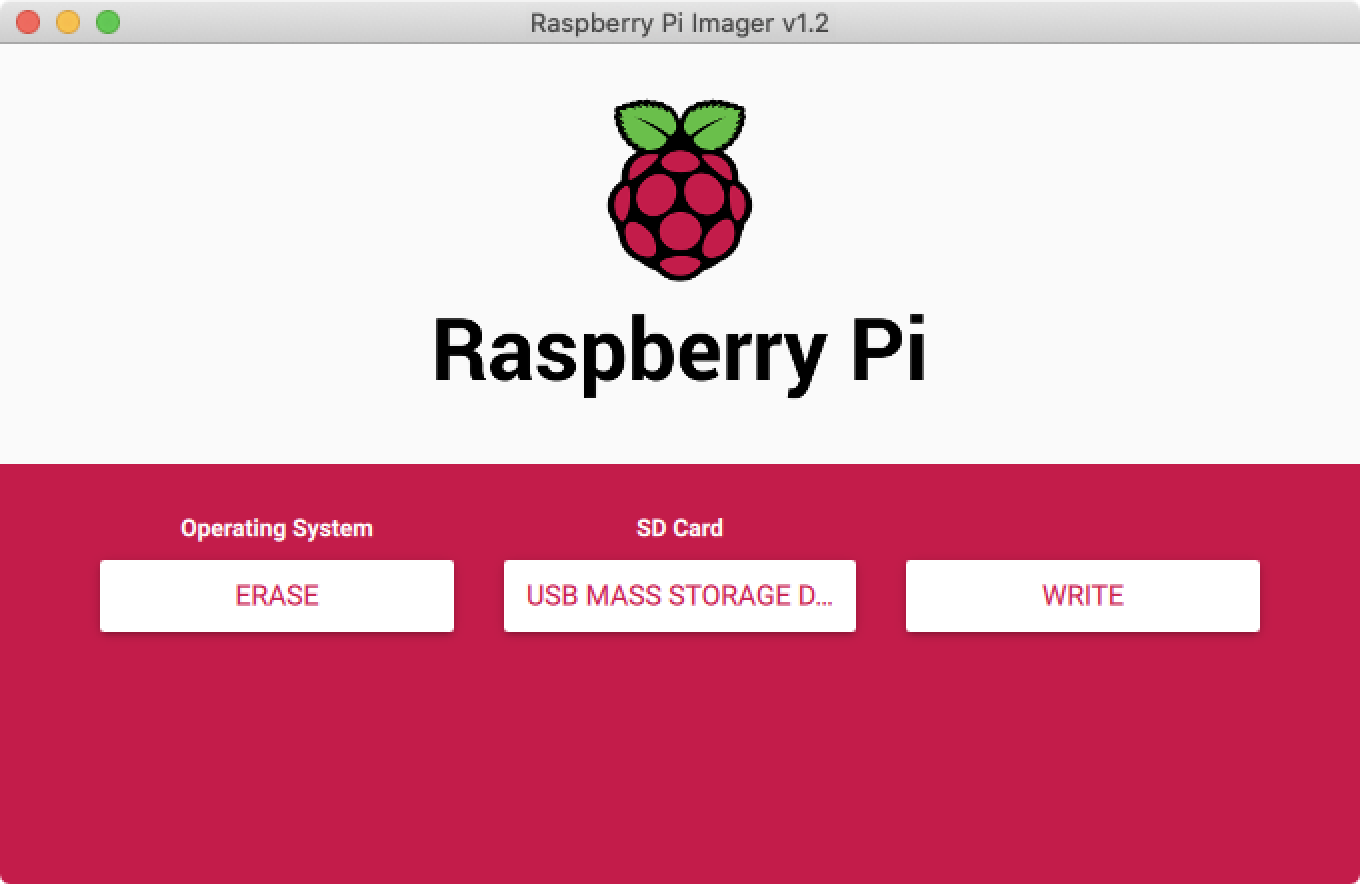
\includegraphics[width=1.0\textwidth]{screenshots/imager-erase.png}
	\caption{Using Raspberry Pi Imager to erase and format a MicroSD card.}
\end{figure}

\begin{figure}[H]
	\centering	
	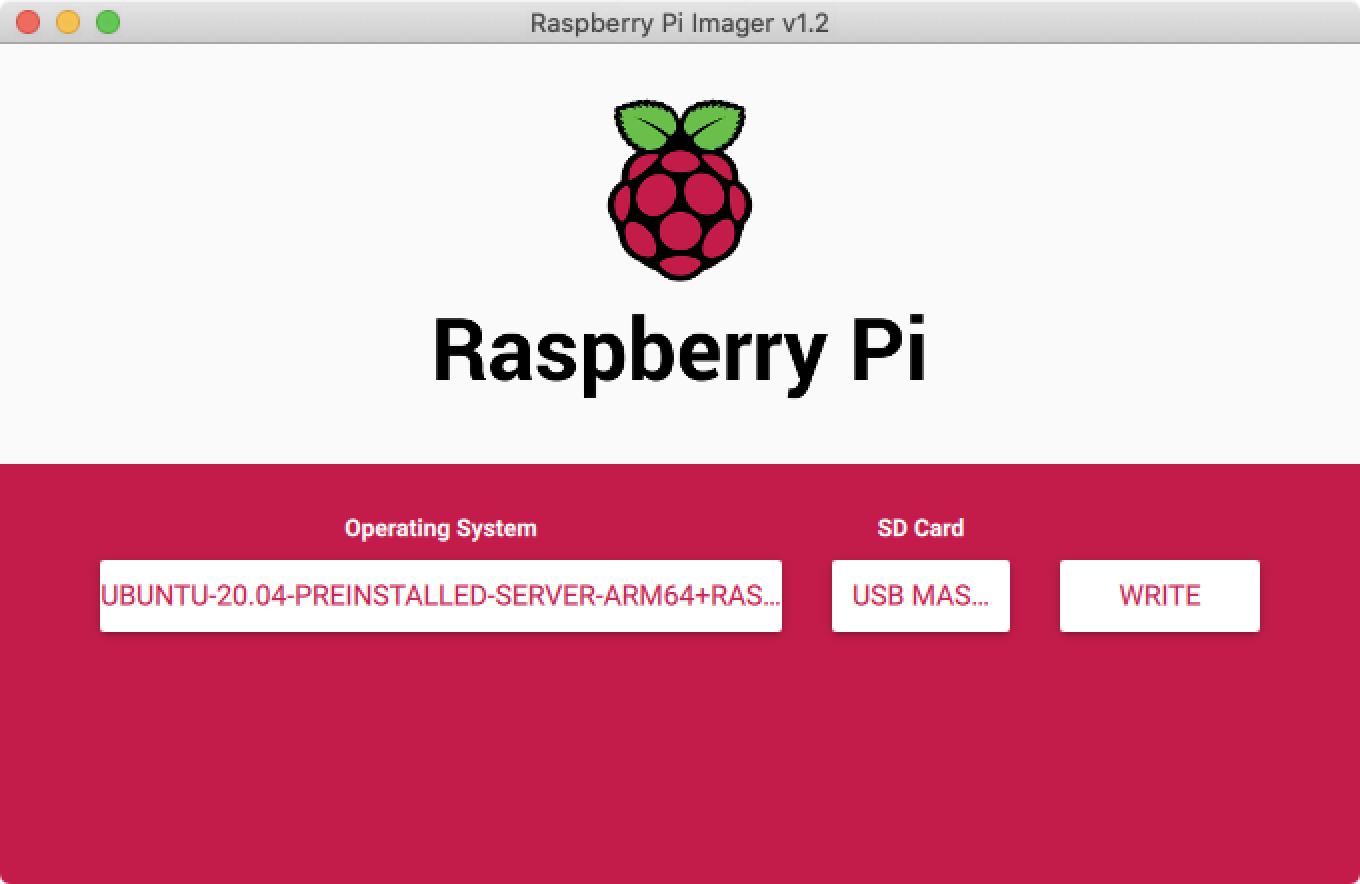
\includegraphics[width=1.0\textwidth]{screenshots/imager-write.png}
	\caption{Using Raspberry Pi Imager to write the server image to a MicroSD card.}
\end{figure}



%
% SECTION
%
\section{Ubuntu Installation}

Having burnt the installation image to each MicroSD card, place the card in each node and plug in the power cable. The \verb|cloud-init| configuration process will now start. Each node will acquire its IP address from the router/firewall, setup system users, update the \verb|apt| cache, upgrade the system, download software packages, set the hostname (based on the IP address), and finally reboot.


%
% SECTION
%
\section{Post-Installation Tasks}


%
% SUB SECTION
%
\subsection{Complete the OpenMPI Password-Less Process}

The user \verb|john|'s public key was installed on each node by \verb|cloud-init|.

It remains to copy the private key to \verb|node1|:

\lstset{style=type}
\begin{lstlisting}
$ scp ~/.ssh/id_rsa node1:~/.ssh
\end{lstlisting}

To complete the process the host keys from \verb|node2| to \verb|node9| need to be imported into the \verb|known_hosts| file of \verb|node1|.

From \verb|macbook|, \verb|ssh| into \verb|node1|:

\lstset{style=type}
\begin{lstlisting}[]
$ ssh node1
\end{lstlisting}

Then from \verb|node1|, \verb|ssh| into \verb|node2| to \verb|node9| in turn, for example:

\lstset{style=type}
\begin{lstlisting}[]
$ ssh node2
\end{lstlisting}


This will generate a message similar to this:

\lstset{style=type}
\begin{lstlisting}[]
The authenticity of host 'node2 (192.168.0.2)' can't be established.
ECDSA key fingerprint is SHA256:5VgsnN2nPvpfbJmALh3aJdOeT/NvDXqN8TCreQyNaFA.
Are you sure you want to continue connecting (yes/no/[fingerprint])?
\end{lstlisting}

Responding \verb|yes| to this this message, imports the \verb|node2| host key into the \verb|~/.ssh/known_hosts| file of \verb|node1|.

Then exit from the connected node:

\lstset{style=type}
\begin{lstlisting}[]
$ exit
\end{lstlisting}

This completes the process.

Subsequent \verb|ssh| access to \verb|node2| to \verb|node9| from \verb|node1| will be done using password-less public key authentication. This is the mechanism that OpenMPI will use.


%
% SUB SECTION
%

\subsection{Uninstall \texttt{unattended-upgrades}}

The \verb|unattended-upgrades| package is installed automatically. This can potentially interfere with long running benchmarks, so it is preferable to uninstall this package from each node. This can be done using Pi Cluster Tools.

From \verb|macbook|:

\lstset{style=type}
\begin{lstlisting}[]
$ ssh node1
$ ~/picluster/tools/do "sudo apt remove unattended-upgrades"
\end{lstlisting}

It is important not to forget to manually upgrade the cluster regularly using Pi Cluster Tools:

\lstset{style=type}
\begin{lstlisting}[]
$ ssh node1
$ ~/picluster/tools/upgrade
\end{lstlisting}



%
% SUB SECTION
%
\subsection{Add Ubuntu Source Repositories}

The Ubuntu source repositories are required to rebuilding the kernel and other Ubuntu packages. These repositories are added as follows:

\lstset{style=type}
\begin{lstlisting}[]
$ ssh node1
$ sudo touch /etc/apt/sources/list.d/picluster.list
\end{lstlisting}

Then add the following to the newly created \verb|picluster.list| file:

\lstset{style=listing}
\begin{lstlisting}[caption=/etc/apt/sources.list.d/picluster.list]
deb-src http://archive.ubuntu.com/ubuntu focal main universe
deb-src http://archive.ubuntu.com/ubuntu focal-updates main universe
\end{lstlisting}

And finally, update the \verb|apt| repository cache:

\lstset{style=type}
\begin{lstlisting}[]
$ sudo apt update
\end{lstlisting}



\subsection{Create a Project Repository}

A project repository on \verb|node1| is required to hold all project software and results. This repository is mirrored with the GitHub project repository.

The project repository is created as follows:

\lstset{style=type}
\begin{lstlisting}[]
$ ssh node1
$ mkdir picluster
$ cd picluster
$ git init
\end{lstlisting}



%
% CHAPTER
%
\chapter{Install High-Performance Linpack (HPL)}

These instructions are derived from the \verb|INSTALL| and \verb|README| files in the \verb|hpl-2.3| top level source directory.

Download and install the latest version of HPL on \verb|node1|:

\lstset{style=type}
\begin{lstlisting}
$ ssh node1
$ cd ~/picluster
$ mkdir hpl
$ cd hpl
$ wget https://www.netlib.org/benchmark/hpl/hpl-2.3.tar.gz
$ gunzip hpl-2.3.tar.gz
$ tar xvf hpl-2.3.tar
$ rm hpl-2.3.tar
$ cd hpl-2.3
\end{lstlisting}

Each computer system requires a specific \verb|Make.picluster| file, which specifies the operating system commands and software package locations required to build HPL. 

Create a generic \verb|Make.picluster| file:

\lstset{style=type}
\begin{lstlisting}
$ cd setup
$ bash make_generic
$ cp Make.UNKNOWN ../Make.picluster
$ cd ..
\end{lstlisting}

Amend \verb|Make.picluster| with the specifics of the Raspberry Pi 4 and Ubuntu 20.04 as follows. The changes below are changes to the generic file created above.

Set the \emph{shell} to use:

\lstset{style=listing}
\begin{lstlisting}[numbers=none]  
SHELL        = /usr/bin/bash
\end{lstlisting}

Set the commands to use (these may vary form operating system to operating system):

\lstset{style=listing}
\begin{lstlisting}[numbers=none]  
CD           = cd
CP           = cp
LN_S         = ln -s
MKDIR        = mkdir -p
RM           = rm -f
TOUCH        = touch
\end{lstlisting}

Set the platform identifier:

\lstset{style=listing}
\begin{lstlisting}[numbers=none]  
ARCH         = picluster
\end{lstlisting}

Set the top level source directory:

\lstset{style=listing}
\begin{lstlisting}[numbers=none]  
TOPdir       = $(HOME)/picluster/hpl/hpl-2.3
\end{lstlisting}

Set the location of the OpenMPI library:

\lstset{style=listing}
\begin{lstlisting}[numbers=none]  
MPdir        = /usr/lib/aarch64-linux-gnu/openmpi
MPinc        = $(MPdir)/include
MPlib        = $(MPdir)/lib/libmpi.so
\end{lstlisting}

Set the location of the BLAS library (Note, this is the location of the Debian \emph{alternatives} \verb|libblas.so.3| library. The actual library that this points to, OpenBLAS or BLIS, is set through the Debian \verb|update-alternatives| command. This can be conveniently done using Pi Cluster Tools.):

\lstset{style=listing}
\begin{lstlisting}[numbers=none]  
LAdir        = /usr/lib/aarch64-linux-gnu
LAinc        =
LAlib        = $(LAdir)/libblas.so.3
\end{lstlisting}

Set the ``Fortran to C'' defintitions, the header directories and libraries: 

\lstset{style=listing}
\begin{lstlisting}[numbers=none]  
F2CDEFS      = -DAdd_ -DF77_INTEGER=int -DStringSunStyle
...
HPL_INCLUDES = -I$(INCdir) -I$(INCdir)/$(ARCH) -I$(MPinc)
HPL_LIBS     = $(HPLlib) $(LAlib) $(MPlib)
...
HPL_DEFS     = $(F2CDEFS) $(HPL_OPTS) $(HPL_INCLUDES)
\end{lstlisting}

And finally, set the compiler, linker and optimisation flags:

\lstset{style=listing}
\begin{lstlisting}[numbers=none]  
CC           = mpicc
CCNOOPT      = $(HPL_DEFS)
CCFLAGS      = $(HPL_DEFS) -O3 -march=armv8-a -mtune=cortex-a72
...
LINKER       = $(CC)
LINKFLAGS    = $(CCFLAGS)
...
ARCHIVER     = ar
ARFLAGS      = r
RANLIB       = echo
\end{lstlisting}

Build HPL:

\lstset{style=type}
\begin{lstlisting}
$ make arch=picluster   
\end{lstlisting}

This creates the executable \verb|xhpl| and input file \verb|HPL.dat| in the \verb|bin/picluster| directory.

The \verb|xhpl| executable has to exist in the same location on each node, so copy \verb|xhpl| to \verb|node2| to \verb|node8| (only \verb|xhpl|, and not \verb|HPL.dat|):

\lstset{style=type}
\begin{lstlisting}
$ cd bin/picluster
$ ~/picluster/tools/do "mkdir -p picluster/hpl/hpl-2.3/bin/picluster"
$ scp xhpl node2:~picluster/hpl/hpl-2.3/bin/picluster
$ scp xhpl node3:~picluster/hpl/hpl-2.3/bin/picluster
$ scp xhpl node4:~picluster/hpl/hpl-2.3/bin/picluster
$ scp xhpl node5:~picluster/hpl/hpl-2.3/bin/picluster
$ scp xhpl node6:~picluster/hpl/hpl-2.3/bin/picluster
$ scp xhpl node7:~picluster/hpl/hpl-2.3/bin/picluster
$ scp xhpl node8:~picluster/hpl/hpl-2.3/bin/picluster
\end{lstlisting}


%
% CHAPTER
%
\chapter{Install HPC Challenge (HPCC)}

These instructions are derived from the README.txt file in the top level directory of the HPCC source code.

It is assumed that HPL has previously been installed, and a HPL build file \verb|Make.picluster| has already been created. This file is copied to the HPCC build directory. See Chapter 8 for the instructions on how to install HPL.

Download and install the latest version of HPCC on \verb|node1|:

\lstset{style=type}
\begin{lstlisting}
$ ssh node1
$ cd ~/picluster
$ mkdir hpcc
$ cd hpcc
$ wget http://icl.cs.utk.edu/projectsfiles/hpcc/download/hpcc-1.5.0.tar.gz
$ gunzip hpcc-1.5.0.tar.gz
$ tar xvf hpcc-1.5.0.tar
$ rm hpcc-1.5.0.tar
$ cd hpcc-1.5.0
\end{lstlisting}

Copy the HPL build script \verb|Make.picluster| to the HPCC \verb|hpl| directory:

\lstset{style=type}
\begin{lstlisting}
$ cd hpl
$ cp ~/picluster/hpl/hpl-2.3/Make.picluster .
\end{lstlisting}

Make the following changes to \verb|Make.picluster|. These differ from the HPL build instructions:

Change the \verb|TOPdir| variable:

\lstset{style=hack}
\begin{lstlisting}[caption=Make.picluster]
TOPdir = ../../..
\end{lstlisting}

Add the \verb|math| library explicitly:

\lstset{style=hack}
\begin{lstlisting}[caption=Make.picluster]
LAlib = $(LAdir)/libblas.so.3 -lm
\end{lstlisting}

Add the constant \verb|OMPI_OMIT_MPI1_COMPAT_DECLS| to \verb|CCFLAGS|, otherwise the compilation will fail:

\lstset{style=hack}
\begin{lstlisting}[caption=Make.picluster]
CCFLAGS = $(HPL_DEFS) -O3 -march=armv8-a -mtune=cortex-a72 -DOMPI_OMIT_MPI1_COMPAT_DECLS
\end{lstlisting}

Move back up into the top level directory:

\lstset{style=type}
\begin{lstlisting}
$ cd ..
\end{lstlisting}

Build HPCC:

\lstset{style=type}
\begin{lstlisting}
$ make arch=picluster
\end{lstlisting}

Copy the \verb|hpcc| executable to the compute nodes:

\lstset{style=type}
\begin{lstlisting}
$ ~/picluster/tools/do "mkdir -p ~/picluster/hpcc/hpcc-1.5.0"
$ scp hpcc node2:~/picluster/hpcc/hpcc-1.5.0
$ scp hpcc node3:~/picluster/hpcc/hpcc-1.5.0
$ scp hpcc node4:~/picluster/hpcc/hpcc-1.5.0
$ scp hpcc node5:~/picluster/hpcc/hpcc-1.5.0
$ scp hpcc node6:~/picluster/hpcc/hpcc-1.5.0
$ scp hpcc node7:~/picluster/hpcc/hpcc-1.5.0
$ scp hpcc node8:~/picluster/hpcc/hpcc-1.5.0
\end{lstlisting}

Create the input file \verb|hpccinf.txt|:

\lstset{style=type}
\begin{lstlisting}
$ cp _hpccinf.txt hpccinf.txt
\end{lstlisting}

The input file is amended as necessary for each benchmark run, as per the HPL input file.

After each benchmark run the results will be in the output file \verb|hpccoutf.txt|.



%
% CHAPTER
%
\chapter{Install High Performance Conjugate Gradients (HPCG)}


%
% CHAPTER
%
\chapter{Ubuntu Kernel Build Procedure}

This procedure is derived from the Ubuntu Wiki BuildYourOwnKernel document...

Make sure you have made the source code repositories available as per...

Create a kernel build directory with the correct directory permissions to prevent source download warnings. 

\lstset{style=type}
\begin{lstlisting}
$ ssh node1
$ mkdir -p ~/picluster/build/kernel
$ sudo chown _apt:root ~/picluster/build/kernel
$ cd ~/picluster/build/kernel
\end{lstlisting}

Install the kernel build dependencies...

\lstset{style=type}
\begin{lstlisting}
$ sudo apt-get build-dep linux linux-image-$(uname -r)
\end{lstlisting}

Download the kernel source...

\lstset{style=type}
\begin{lstlisting}
$ sudo apt-get source linux-image-$(uname -r)
$ cd linux-raspi-5.4.0
\end{lstlisting}

This bit is a fix for the subsequent \verb|editconfigs| step of the build procedure...

\lstset{style=type}
\begin{lstlisting}
$ cd debian.raspi/etc
$ sudo cp kernelconfig kernelconfig.original
$ sudo vim kernelconfig
\end{lstlisting}

And make the following change...

\lstset{style=listing}
\begin{lstlisting}[caption=diff kernelconfig kernelconfig.original, numbers=none]
5c5
< 	archs="arm64"
---
> 	archs="armhf arm64"
\end{lstlisting}

Then move back up to the kernel source top level directory...

\lstset{style=type}
\begin{lstlisting}
$ cd ../..
\end{lstlisting}

Prepare the build scripts...

\lstset{style=type}
\begin{lstlisting}
$ sudo chmod a+x debian/rules
$ sudo chmod a+x debian/scripts/*
$ sudo chmod a+x debian/scripts/misc/*
\end{lstlisting}

SOURCE CHANGES AND/OR verb|editconfigs| AT THIS POINT

\lstset{style=type}
\begin{lstlisting}
$ sudo apt install libncurses-dev
$ sudo LANG=C fakeroot debian/rules clean
$ sudo LANG=C fakeroot debian/rules editconfigs
\end{lstlisting}

Tweak the kernel name for identification...

\lstset{style=type}
\begin{lstlisting}
$ cd debian.raspi
$ sudo cp changelog changelog.original
$ sudo vim changelog
\end{lstlisting}

And make the following change, where \verb|+picluster0| is our kernel identifier...

\lstset{style=listing}
\begin{lstlisting}[caption=diff changelog changelog.original, numbers=none]
1c1
< linux-raspi (5.4.0-1015.15+picluster0) focal; urgency=medium
---
> linux-raspi (5.4.0-1015.15) focal; urgency=medium
\end{lstlisting}

Move up to the top level kernel source directory...

\lstset{style=type}
\begin{lstlisting}
$ cd ..
\end{lstlisting}

And build the kernel...

\lstset{style=type}
\begin{lstlisting}
$ sudo LANG=C fakeroot debian/rules clean
$ sudo LANG=C fakeroot debian/rules binary-arch
cd ..
\end{lstlisting}

Install the new kernel...

\lstset{style=type}
\begin{lstlisting}
$ sudo dpkg -i linux*picluster0*.deb
$ sudo shutdown -r now
\end{lstlisting}

Another build procedure fix...

After each kernel build delete the \verb|linux-libc-dev| directory...

\lstset{style=type}
\begin{lstlisting}
$ cd ~/picluster/build/kernel/linux-raspi-5.4.0/debian
$ rm -rf linux-libc-dev
$ cd ..
\end{lstlisting}


%
% CHAPTER
%
\chapter{Build Kernel with No Pre-Emption Scheduler}


%
% CHAPTER
%
\chapter{Build Kernel with Jumbo Frames Support}

Standard MTU is 1500 bytes...

Maximum payload size is 1472 bytes...

NB of 184 (x 8 bytes for Double Precision) = 1472 bytes...

NB $>$ 184 $=>$ packet fragmentation $=>$ reduced network efficiency...

This causes drop of in performance???...

Max MTU on Raspberry Pi 4 Model B is set at build time to 1500...

Not configurable above 1500...

TODO: EXAMPLE OF ERROR MSG...

Need to build the kernel with higher MTU...


Make the required changes to the source... as per REFERENCE

\begin{verbatim}
    cd linux-raspi-5.4.0 

    sudo vim include/linux/if_vlan.h...
        #define VLAN_ETH_DATA_LEN   9000
        #define VLAN_ETH_FRAME_LEN  9018
    
    sudo vim include/uapi/linux/if_ether.h...
        #define ETH_DATA_LEN        9000
        #define ETH_FRAME_LEN       9014
    
    sudo vim drivers/net/ethernet/broadcom/genet/bcmgenet.c...
        #define RX_BUF_LENGTH       10240
\end{verbatim}

Add a Jumbo Frames identifier, "+jf", to the new kernel name...

\begin{verbatim}
    sudo vim debian.raspi/changelog...
        linux (5.4.0-1013.13+jf) focal; urgency=medium
        
\end{verbatim}


%
% CHAPTER
%
\chapter{Rebuild OpenBLAS}

\lstset{style=type}
\begin{lstlisting}
$ ssh node1
$ mkdir -p build/openblas
$ chown -R _apt:root build
$ cd build/openblas
$ sudo apt-get source openblas
$ sudo apt-get build-dep openblas
$ cd openblas-0.3.8+ds
\end{lstlisting}


Edit cpuid\_arm64.c...

\lstset{style=type}
\begin{lstlisting}
$ sudo cp cpuid_arm64.c cpuid_arm64.c.original
$ sudo vim cpuid_arm64.c
\end{lstlisting}


\lstset{style=type}
\begin{lstlisting}
$ diff cpuid_arm64.c cpuid_arm64.c.original
\end{lstlisting}

\lstset{style=type}
\begin{lstlisting}
275c275
<       printf("#define L2_SIZE 1048576\n");
---
>       printf("#define L2_SIZE 524288\n");
278c278
<       printf("#define DTB_DEFAULT_ENTRIES 32\n");
---
>       printf("#define DTB_DEFAULT_ENTRIES 64\n");
\end{lstlisting}


And, then following the instructions in debian/README.Debian

\lstset{style=type}
\begin{lstlisting}
$ DEB_BUILD_OPTIONS=custom dpkg-buildpackage -uc -b
\end{lstlisting}

Once the build is complete..

\lstset{style=type}
\begin{lstlisting}
cd ..
$ sudo apt remove libopenblas0-serial
$ sudo dpkg -i libopenblas0-serial\_0.3.8+ds-1\_arm64.deb
\end{lstlisting}

Ensure the correct BLAS library is being used...

\lstset{style=type}
\begin{lstlisting}
$ sudo update-alternatives --config libblas.so.3-aarch64-linux-gnu
\end{lstlisting}

copy to other nodes
remove old...
install new...

If more than one BLAS library is installed, check update-alternatives!!!

ssh node2 .. node8
\lstset{style=type}
\begin{lstlisting}
$ ssh node2 sudo apt remove libblas0-serial
$ scp libopenblas0-serial\_0.3.8+ds-1\_arm64.deb node2:~
$ ssh sudo dpkg -i libopenblas0-serial\_0.3.8+ds-1\_arm64.deb
$ ssh sudo update-alternatives --config libblas.so.3-aarch64-linux-gnu
\end{lstlisting}


%
% CHAPTER
%
\chapter{Rebuild BLIS}

\lstset{style=type}
\begin{lstlisting}
$ ssh node1
$ mkdir -p picluster/build/blis
$ cd picluster/build/blis
$ apt-get source blis
$ sudo apt-get build-dep blis
$ cd blis-0.6.1
\end{lstlisting}


%
% CHAPTER
%

\chapter{Build OpenMPI from Source}

Do all of this on node1...

\lstset{style=type}
\begin{lstlisting}
$ ssh node1
\end{lstlisting}

We want to avoid collisions with multiple OpenMPI installations, so remove original installed version...

\lstset{style=type}
\begin{lstlisting}
$ sudo apt remove openmpi-common
$ sudo apt remove openmpi-bin
$ sudo apt autoremove 
\end{lstlisting}

OpenMPI requires the libevent-dev package...

\lstset{style=type}
\begin{lstlisting}
$ sudo apt install libevent-dev
\end{lstlisting}

Create a build directory, and download and, and and following BLAH, BLAH build OpenMPI...

\lstset{style=type}
\begin{lstlisting}
$ mkdir -p ~/picluster/build/openmpi
$ cd ~/picluster/build/openmpi
$ wget https://download.open-mpi.org/release/open-mpi/v4.0/openmpi-4.0.4.tar.gz
$ gunzip openmpi-4.0.4.tar.gz
$ tar xvf openmpi-4.0.4.tar
$ rm openmpi-4.0.4.tar
$ cd openmpi-4.0.4
$ mkdir build
$ cd build
$ ../configure CFLAGS="-O3 -march=armv8-a -mtune=cortex=a72"
$ make all
$ sudo make install
$ sudo ldconfig
\end{lstlisting}

OpenMPI will installed to /usr/local

EXTRACT FROM HPL.dat


TODO: HOW TO COPY TO ALL NODES!


%
% CHAPTER
%
\chapter{Aerin Cluster Tools}

\lstinputlisting[caption=picluster/tools/upgrade, numbers=left, backgroundcolor=\color{LightSkyBlue}]{picluster/tools/upgrade}
\lstinputlisting[caption=picluster/tools/reboot, numbers=left, backgroundcolor=\color{LightSkyBlue}]{picluster/tools/reboot}
\lstinputlisting[caption=picluster/tools/shutdown, numbers=left, backgroundcolor=\color{LightSkyBlue}]{picluster/tools/shutdown}
\lstinputlisting[caption=picluster/tools/libblas-query, numbers=left, backgroundcolor=\color{LightSkyBlue}]{picluster/tools/libblas-query}
\lstinputlisting[caption=picluster/tools/libblas-set, numbers=left, backgroundcolor=\color{LightSkyBlue}]{picluster/tools/libblas-set}


%
% CHAPTER
%

\chapter{Arm Performance Libraries}

\textcolor{red}{This does not work, yet! HPL will compile and link to Arm Performance Libraries, but raises an illegal instruction error at runtime.}

\textcolor{red}{At the time of writing, Arm Performance Libraries release 20.2.0 requires a minimum Instruction Set Architecture (ISA) of armv8.1-a. Unfortunately, the Raspberry Pi's Cortex-A72 ISA is armv8.0-a. An Arm representative has indicated on the Arm HPC Forum that the next release of the libraries will support the armv8.0-a ISA.}

\textcolor{red}{This Chapter is included for future reference.}

The Arm Performance Libraries website states:

"Arm Performance Libraries provides optimised standard core math libraries for high-performance computing applications on Arm processors. This free version of the libraries provides optimised libraries for Arm® Neoverse™ N1-based Armv8 AArch64 implementations that are compatible with various versions of GCC. You do not require a license for this version of the libraries."

To install Arm Performance Libraries, firstly downloaded Arm Performance Libraries 20.2.0 with GCC 9.3 for Ubuntu 16.04+ from the Arm website.

Then follow these instructions.

\lstset{style=type}
\begin{lstlisting}
$ ssh node1
\end{lstlisting}

Install the required \verb|environment_modules| package.

\lstset{style=type}
\begin{lstlisting}
$ sudo apt install environment-modules
\end{lstlisting}

Then extract and install Arm Performance Libraries.

The default installation directory is /opt/arm.

\lstset{style=type}
\begin{lstlisting}
$ mkdir ~/picluster/armpl
$ cd ~/picluster/armpl
$ tar xvf arm-performance-libraries_20.2_Ubuntu-16.04_gcc-9.3.tar
$ rm arm-performance-libraries_20.2_Ubuntu-16.04_gcc-9.3.tar
$ sudo ./arm-performance-libraries_20.2_Ubuntu-16.04.sh
\end{lstlisting}

Copy the \verb|Make.picluster| configuration file.

\lstset{style=type}
\begin{lstlisting}
$ cd ~/picluster/hpl/hpl-2.3
$ cp Make.picluster Make.picluster-armpl
\end{lstlisting}

Make the following changes to \verb|Make.picluster-armpl|.

\lstset{style=listing}
\begin{lstlisting}[caption=Make.picluster-armpl, numbers=none]
LAdir        = /opt/arm/armpl_20.2_gcc-9.3
LAinc        =
LAlib        = -L$(LAdir)/lib -larmpl -lgfortran -lamath -lm
\end{lstlisting}

Build HPL.

\lstset{style=type}
\begin{lstlisting}
$ make arch=picluster-armpl
\end{lstlisting}


%
% THE END
%
\end{document}
